\documentclass[serif]{beamer}

% 中文支持(Overleaf 推荐用思源宋体)
\usepackage{xeCJK}
\setCJKmainfont{Noto Serif CJK SC}

% 数学、图片、代码支持
\usepackage{amsmath, amssymb}
\usepackage{graphicx}
\usepackage{xcolor}
\usepackage{tcolorbox}
\tcbuselibrary{listingsutf8}
\usepackage{listings}
\lstdefinelanguage{json}{
    basicstyle=\ttfamily\footnotesize,
    numbers=left,
    numberstyle=\tiny,
    stepnumber=1,
    numbersep=5pt,
    showstringspaces=false,
    breaklines=true,
    frame=single,
    morestring=[b]",
    stringstyle=\color{red},
    literate=
     *{:}{{{\color{black}:}}}{1}
      {,}{{{\color{black},}}}{1}
      {[}{{{\color{blue}[}}}{1}
      {]}{{{\color{blue}]}}}{1}
      {{\{}{{{\color{blue}\{}}}{1}
      {{\}}}{{{\color{blue}\}}}}{1}
}
\usepackage{xcolor}

% Beamer主题配置
\usetheme{Madrid}
\usecolortheme{whale}
\usefonttheme{professionalfonts}
\usefonttheme[onlymath]{serif}
\setbeamertemplate{navigation symbols}{}

% 自定义页脚样式
\setbeamertemplate{footline}{
  \leavevmode%
  \hbox{%
    \begin{beamercolorbox}[wd=.8\paperwidth,ht=2.25ex,dp=1ex,left]{author in head/foot}
      \usebeamerfont{author in head/foot}\hspace{1em}\insertshorttitle
    \end{beamercolorbox}%
    \begin{beamercolorbox}[wd=.2\paperwidth,ht=2.25ex,dp=1ex,right]{date in head/foot}
      \usebeamerfont{date in head/foot}\insertframenumber{} / \inserttotalframenumber\hspace{1em}
    \end{beamercolorbox}
  }%
  \vskip0pt%
}

% 代码高亮设置
\lstset{
    basicstyle=\ttfamily\footnotesize,
    keywordstyle=\color{blue},
    commentstyle=\color{gray},
    stringstyle=\color{red},
    numbers=left,
    numberstyle=\tiny,
    stepnumber=1,
    numbersep=5pt,
    frame=single,
    breaklines=true,
    captionpos=b
}

% 文档信息(请替换)
\title{创新实践项目答辩}
\author{12310520芮煜涵 \and 12310437乔诗涵}
\institute{南方科技大学  \and 计算机科学与工程系}
\date{\today}

\begin{document}

\begin{frame}
  \titlepage
\end{frame}

\begin{frame}{目录}
  \tableofcontents
\end{frame}



\begin{frame}{工作流程图}
   \begin{figure}
        \centering
        \includegraphics[width=0.95\linewidth]{images/workflow.jpg}
        \caption{Workflow}
        \label{fig:enter-label}
    \end{figure} 
\end{frame}
\section{选题背景与面临的问题}

\begin{frame}{选题背景与面临的问题}
\vspace{-0.4em}
\textbf{选题背景}

\begin{itemize}
\item 采集自动驾驶的视频时会得到大量的数据
\item 但在自动驾驶安全测试中,只需关注\textbf{一小部分特殊情况}(如超车或出现障碍物等危险场景)
\end{itemize}

\textbf{为从大量数据中得到所需数据,需效果良好的视频检索方法}

\vspace{0.4em}

\textbf{面临的问题}
\begin{itemize}
    \item \textbf{自动驾驶视频数据} \\
          自动驾驶领域公开的带有高质量标注的视频数据较少,模型难以通过有限数据准确理解视频内容。
          
          同时,自动驾驶视频与通用视频数据集存在\textbf{较大差异}。
    \item \textbf{自动驾驶视频特点} \\
          自动驾驶视频\textbf{高度依赖帧间关联},画面中物体众多但有效信息稀疏。模型需要识别关键内容,避免被无关物体干扰。
\end{itemize}


\end{frame}



\section{相关工作}

\begin{frame}{相关工作(一):自动驾驶场景数据集描述的自动生成}

\begin{minipage}[t]{0.48\linewidth}
  \centering
  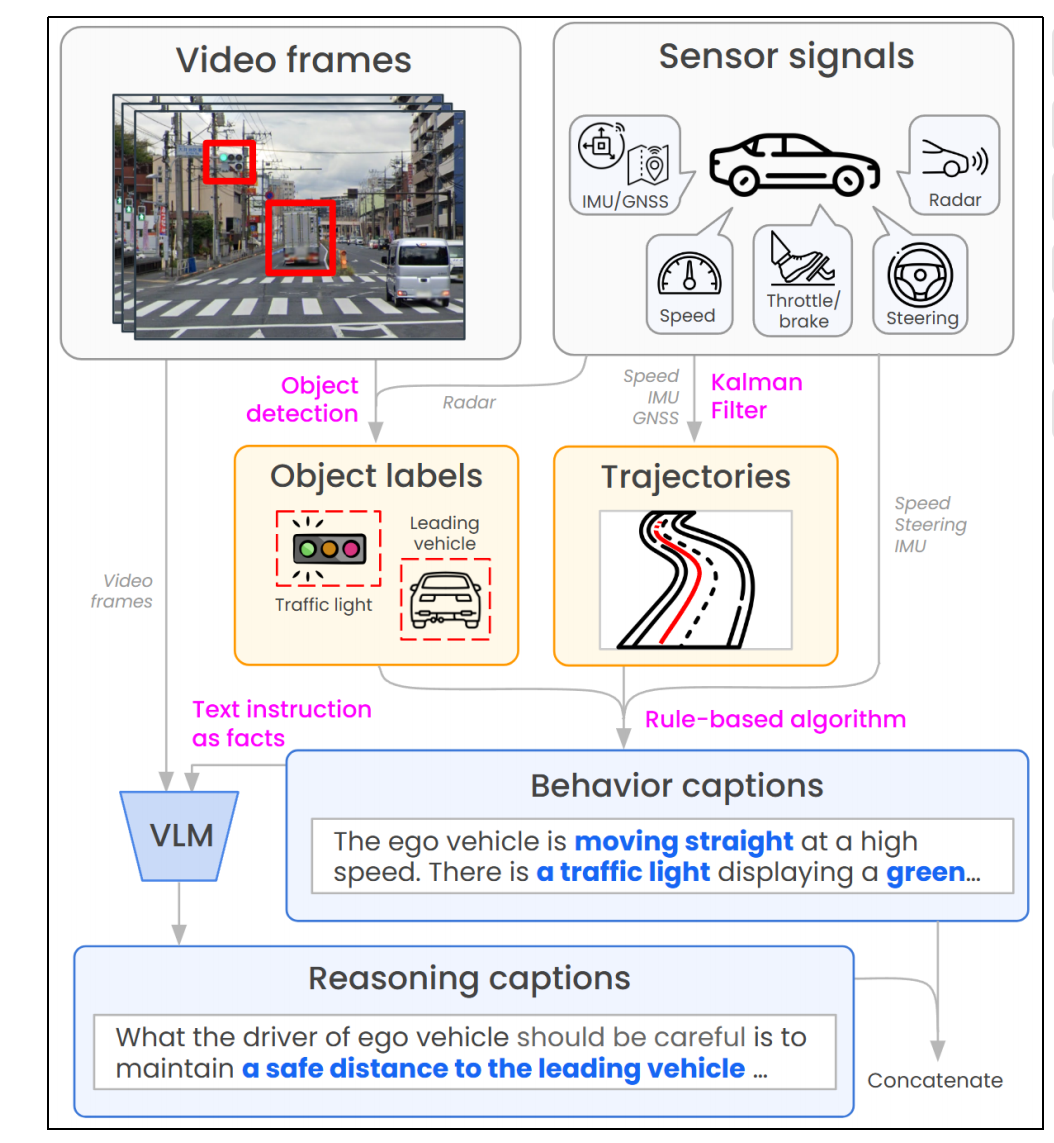
\includegraphics[width=\linewidth]{images/CoVLA.png}
  \caption{CoVLA 数据集描述生成}
\end{minipage}
\hfill
\vspace{1em} % 你也可以调整这个数值微调整体位置
\begin{minipage}[c]{0.48\linewidth} % 注意这里改成了 c
  \vspace{-15em} % 给右侧内容加点垂直空白,让它往上移一点
  \begin{itemize}
  \item \textbf{多传感器融合}:结合视频帧、雷达、IMU等多源数据,实现多模态信息协同
  \item 基于规则算法:利用轨迹和物体检测生成行为描述
  \item 视觉语言模型(VLM):辅助生成行为与推理字幕
  \item \textbf{行为与推理分离}:区分车辆行为和驾驶员注意事项
  \item 目标:自动生成高质量且语义丰富的自动驾驶数据集描述
\end{itemize}

\end{minipage}


\end{frame}



\begin{frame}{相关工作(二):自动驾驶场景数据集与多模态大模型}
\centering
\begin{minipage}{0.9\linewidth}
  \centering
  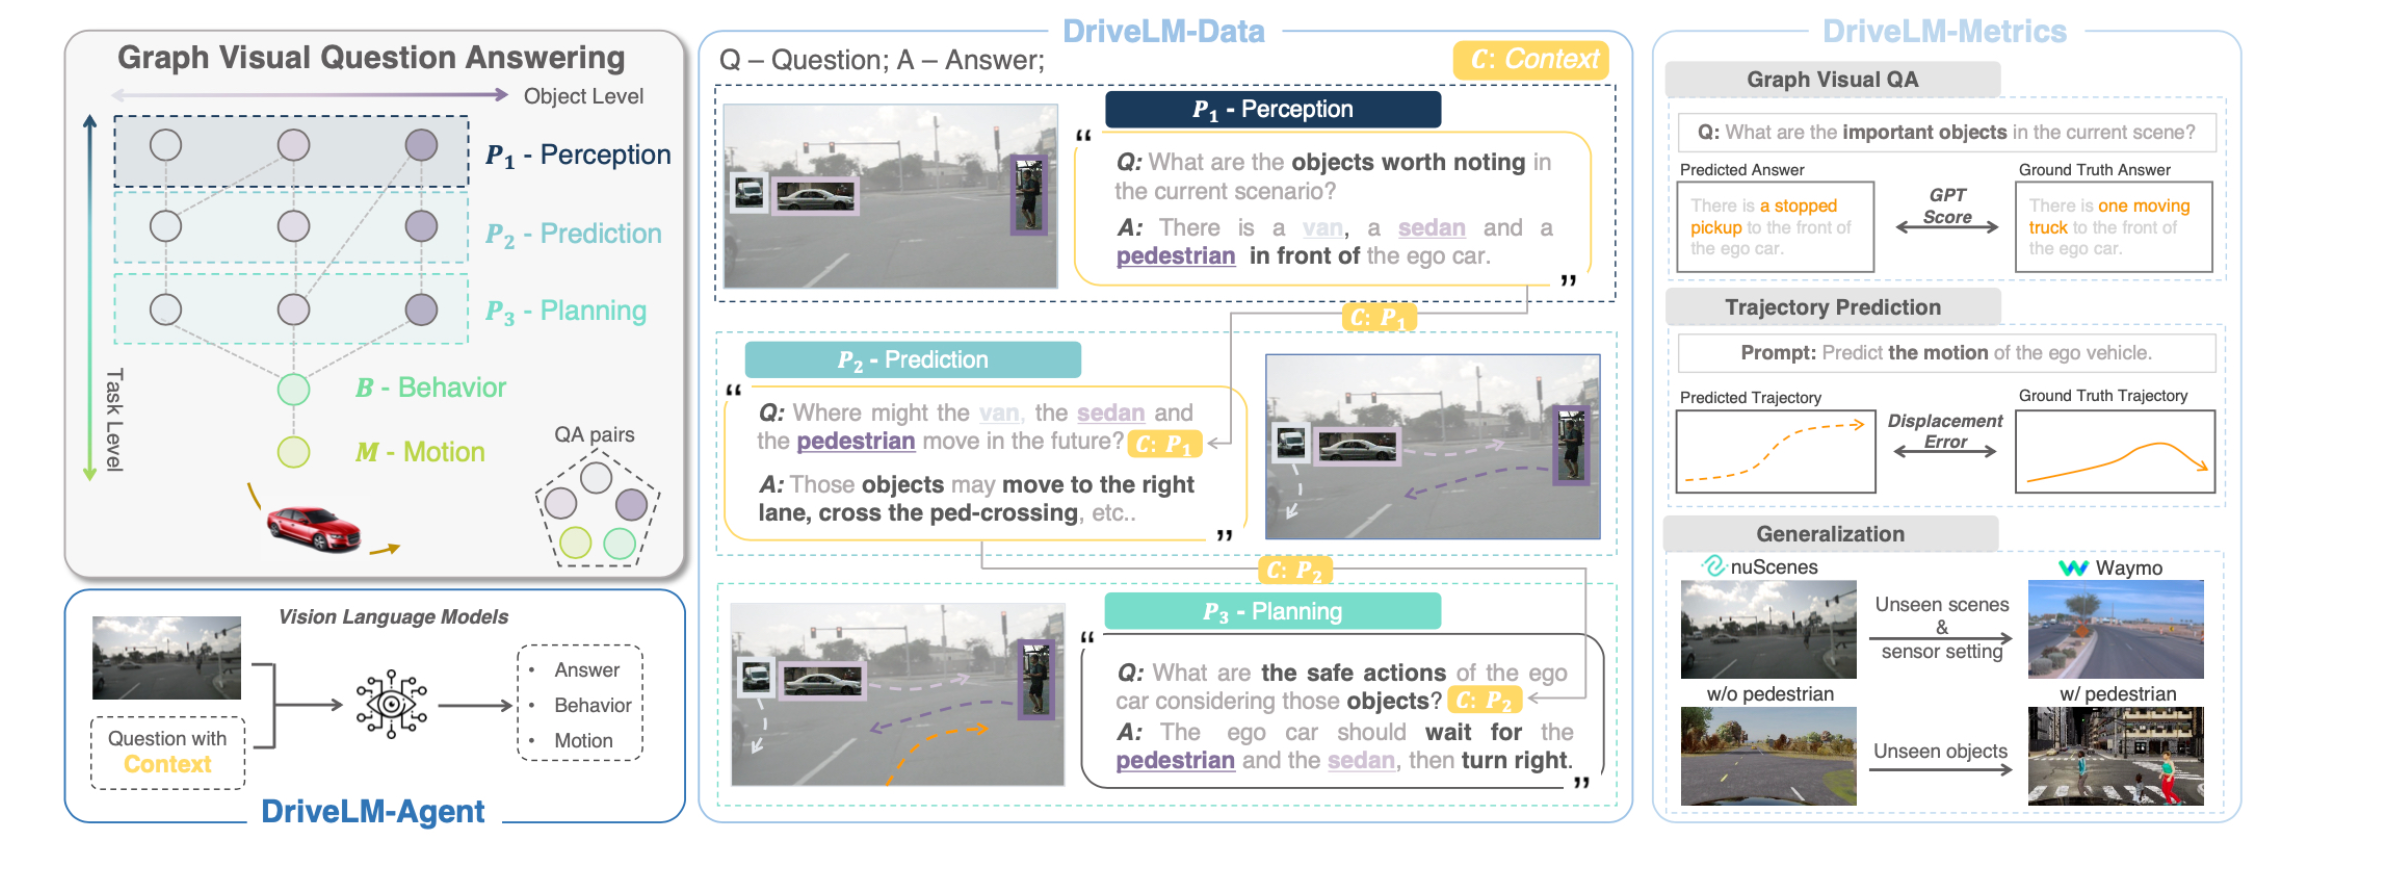
\includegraphics[width=\linewidth]{images/DriveLM.png}
  
  {\footnotesize DriveLM 思维链示例}
\end{minipage}
\vspace{1em}
\begin{flushleft}
    \textbf{针对自动驾驶场景数据集的多模态大模型}
\end{flushleft}


\begin{itemize}
    \item 暂时缺少针对\textbf{自动驾驶场景}数据集的\textbf{开源多模态大模型}
    \item 因此使用\textbf{通用多模态大语言模型}
\end{itemize}
    
\end{frame}

% -----------------------------
\section{视频-文本检索模型}

\begin{frame}{视频-文本检索模型(1):VAST}

采用两种\textbf{视频-文本双向检索}模型,以理解自动驾驶场景中的语义内容:

\vspace{0.2em}

\textbf{VAST}(ECCV 2022)  
\begin{itemize}
  \item 同时处理视觉、字幕、音频和文本多模态;
  \item 视觉(ViT),音频(BEATs),文本编码器(BERT),通过\textbf{跨注意力层}实现多模态融合;
  \item 在多模态视频-文本任务中表现突出。
\end{itemize}

\vspace{0.2em}
\centering
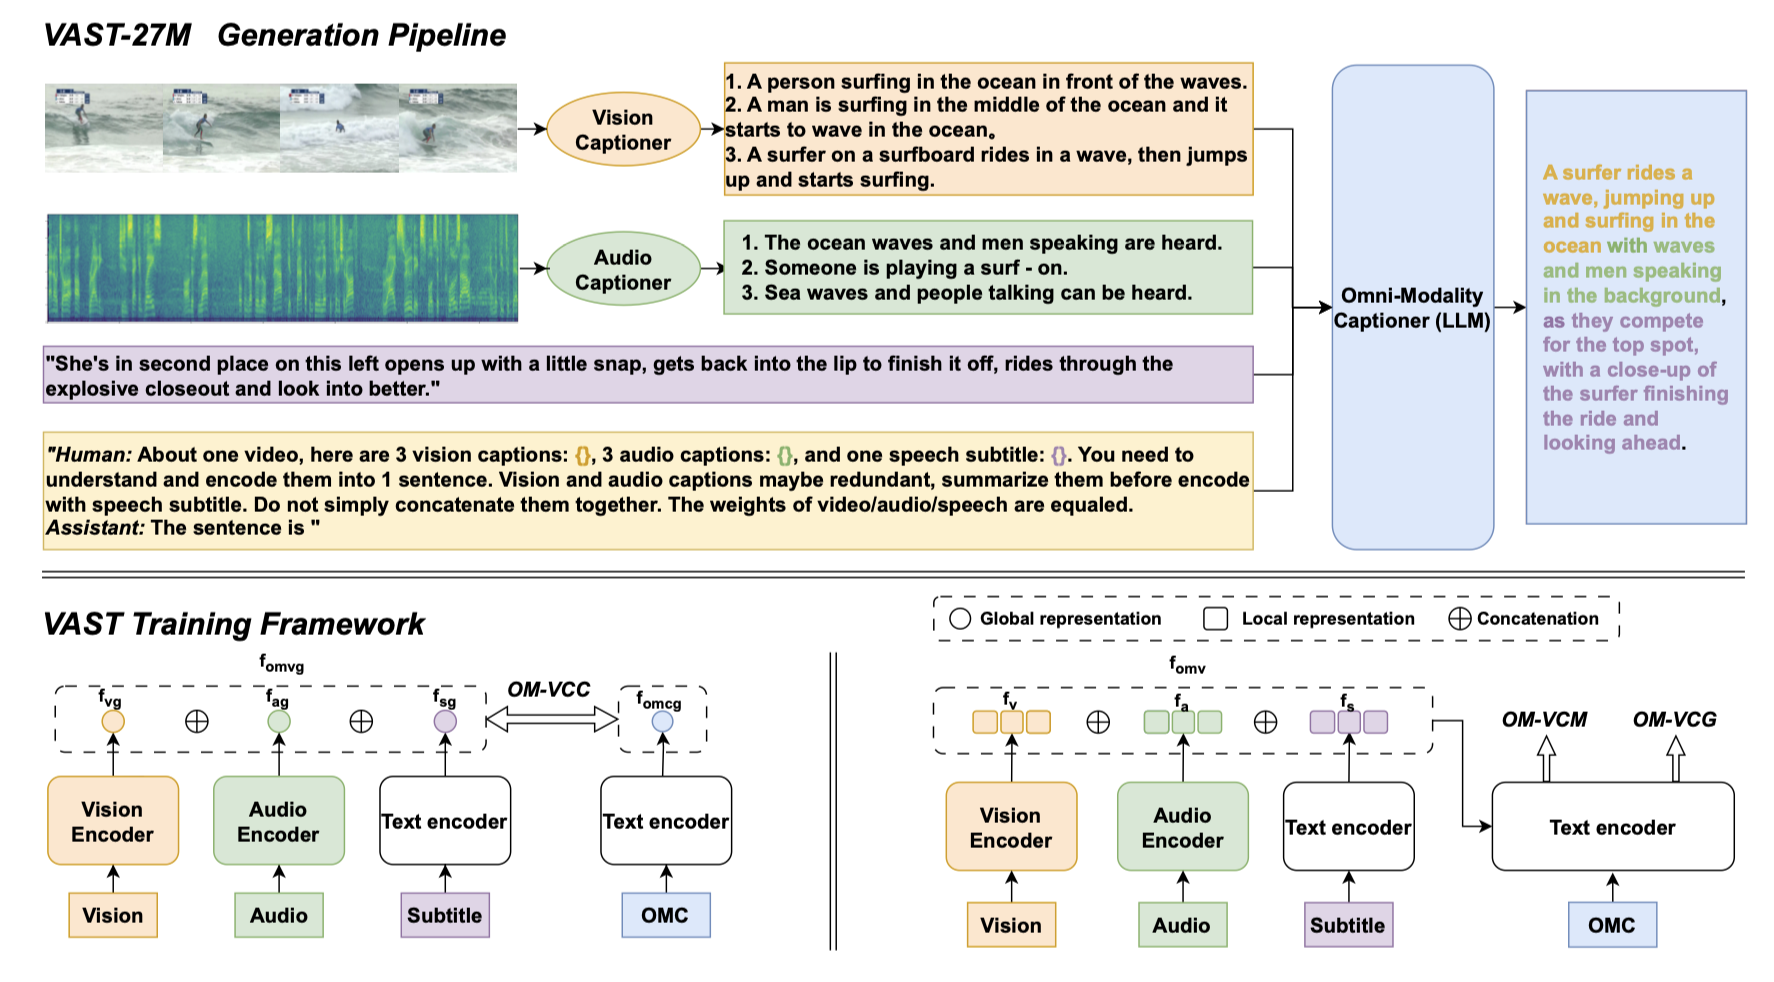
\includegraphics[width=0.75\textwidth]{images/vast_structure.png}\\
{\footnotesize 图:VAST 模型结构}

\end{frame}


\begin{frame}{视频-文本检索模型(2):CLIP-ViP}

采用两种\textbf{视频-文本双向检索}模型,以理解自动驾驶场景中的语义内容:

\vspace{0.2em}

\textbf{CLIP-ViP}(CVPR 2023)  
\begin{itemize}
  \item 基于CLIP的ViT视觉编码器+代理令牌(proxy tokens)实现视频时序建模
  \item \textbf{代理引导注意力}:代理令牌与所有帧交互,帧内patch局部交互
  \item 多源对比学习同时利用视频字幕与辅助帧图像字幕
\end{itemize}

\vspace{0.2em}
\centering
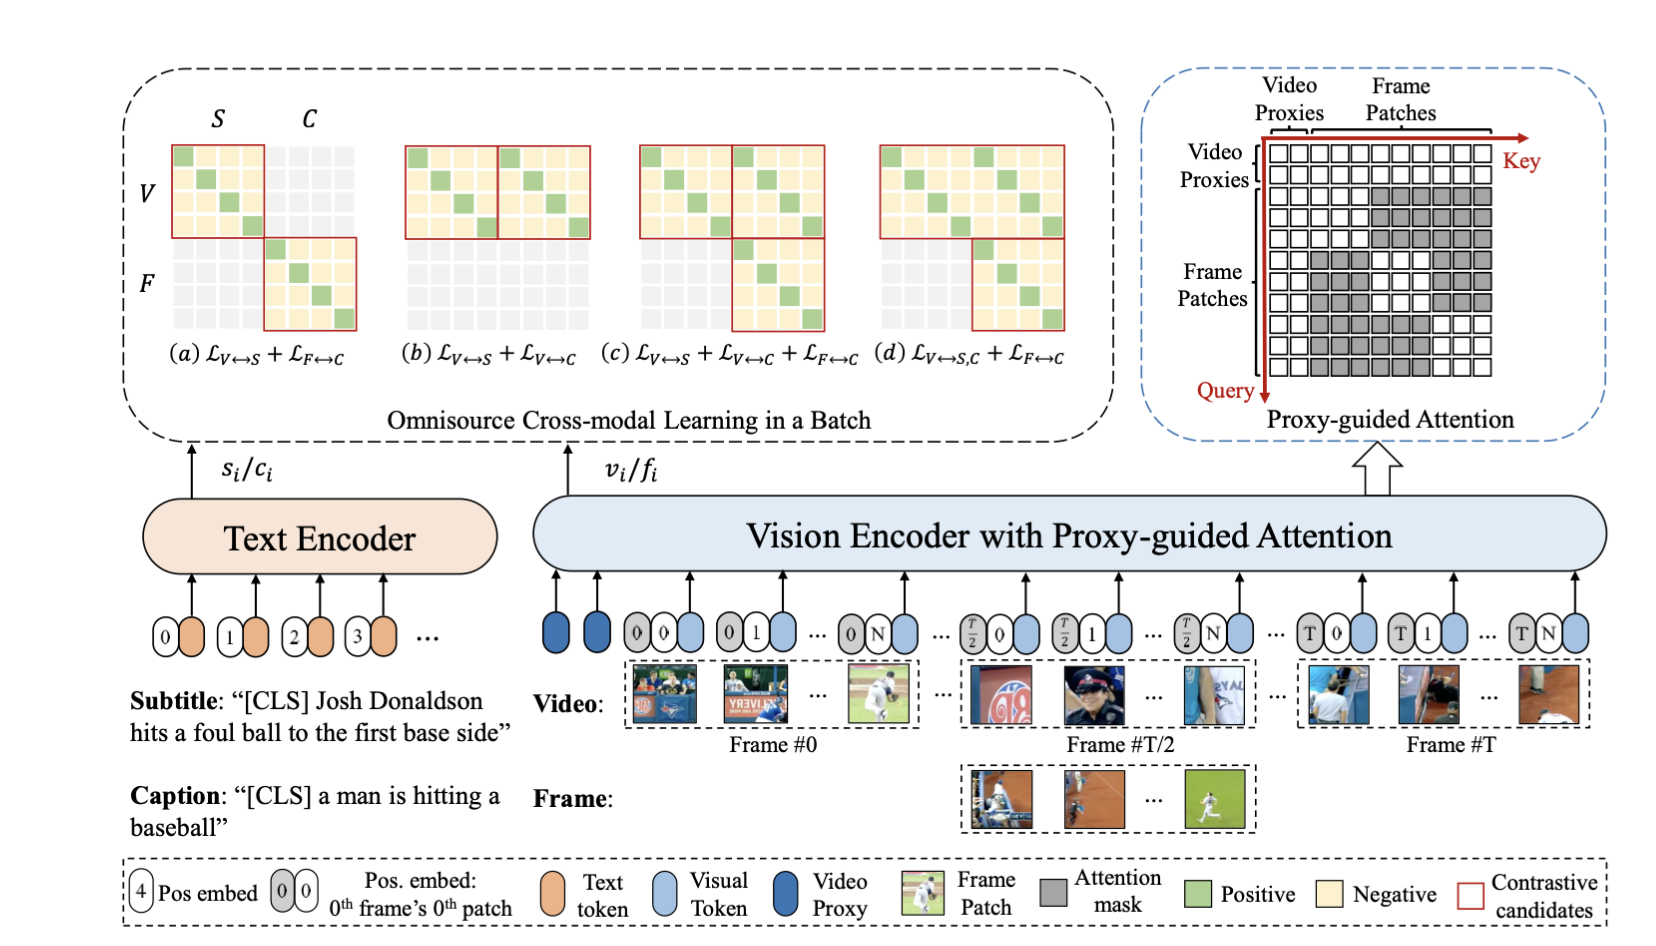
\includegraphics[width=0.75\textwidth]{images/clipvip_structure.png}\\
{\footnotesize 图:CLIP-ViP 模型结构}

\end{frame}

%-------------------------------------
\section{场景描述}

\begin{frame}{数据集:Suscape 数据集与标注形式}

% 图片区域(不修改)
\begin{center}
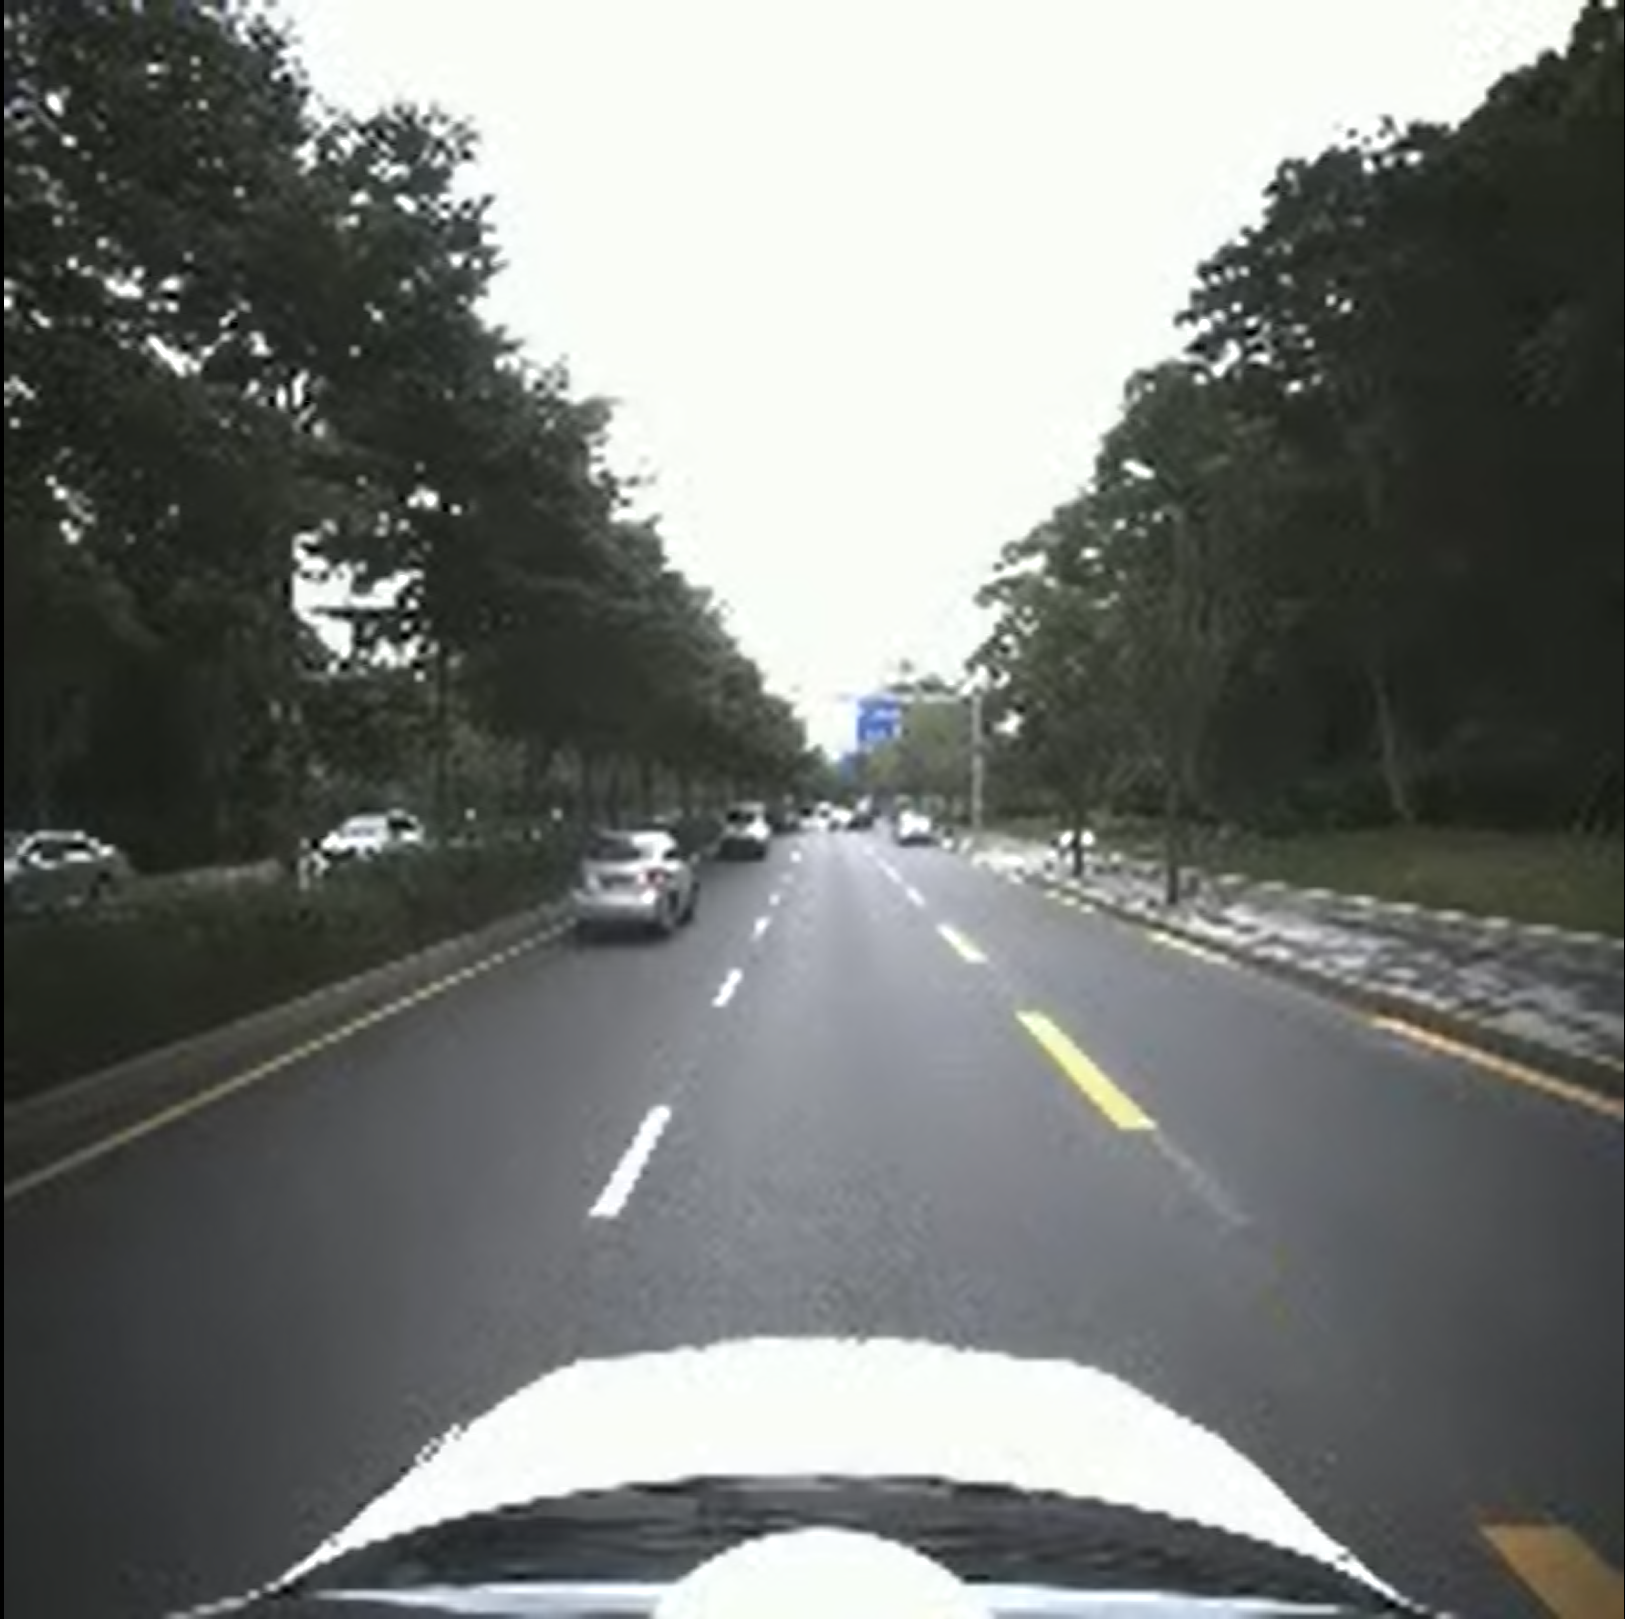
\includegraphics[width=0.20\textwidth]{images/drive_scene1.jpg}
\hfill
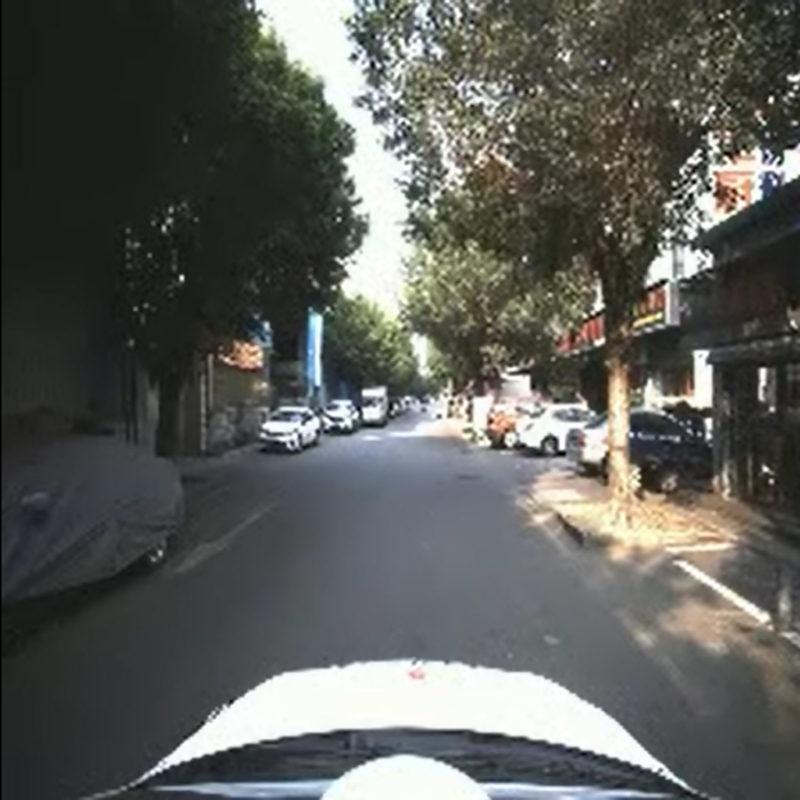
\includegraphics[width=0.20\textwidth]{images/drive_scene2.jpg}
\hfill
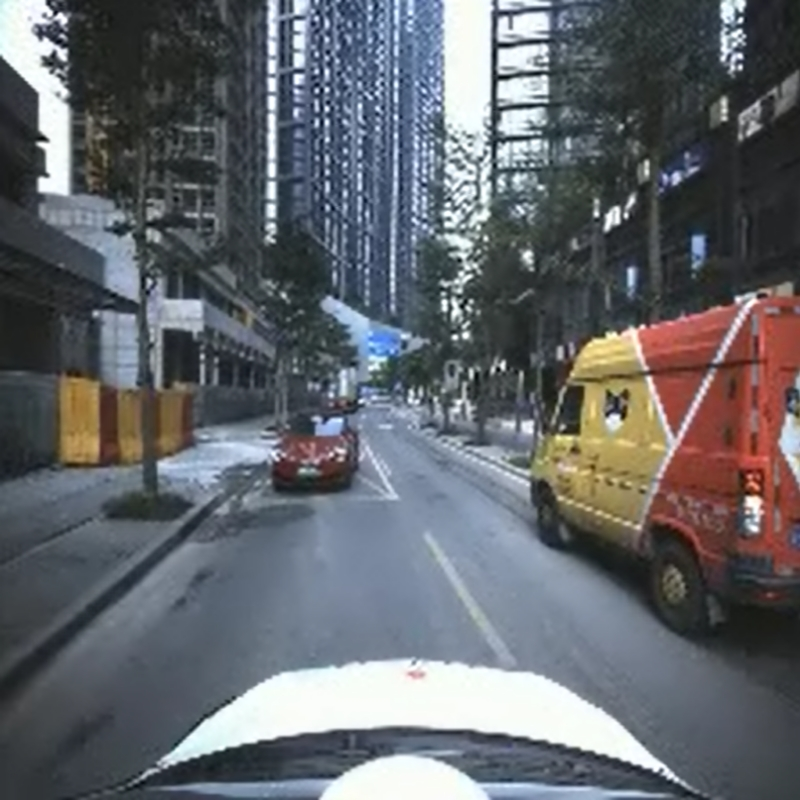
\includegraphics[width=0.20\textwidth]{images/drive_scene3.jpg}
\hfill
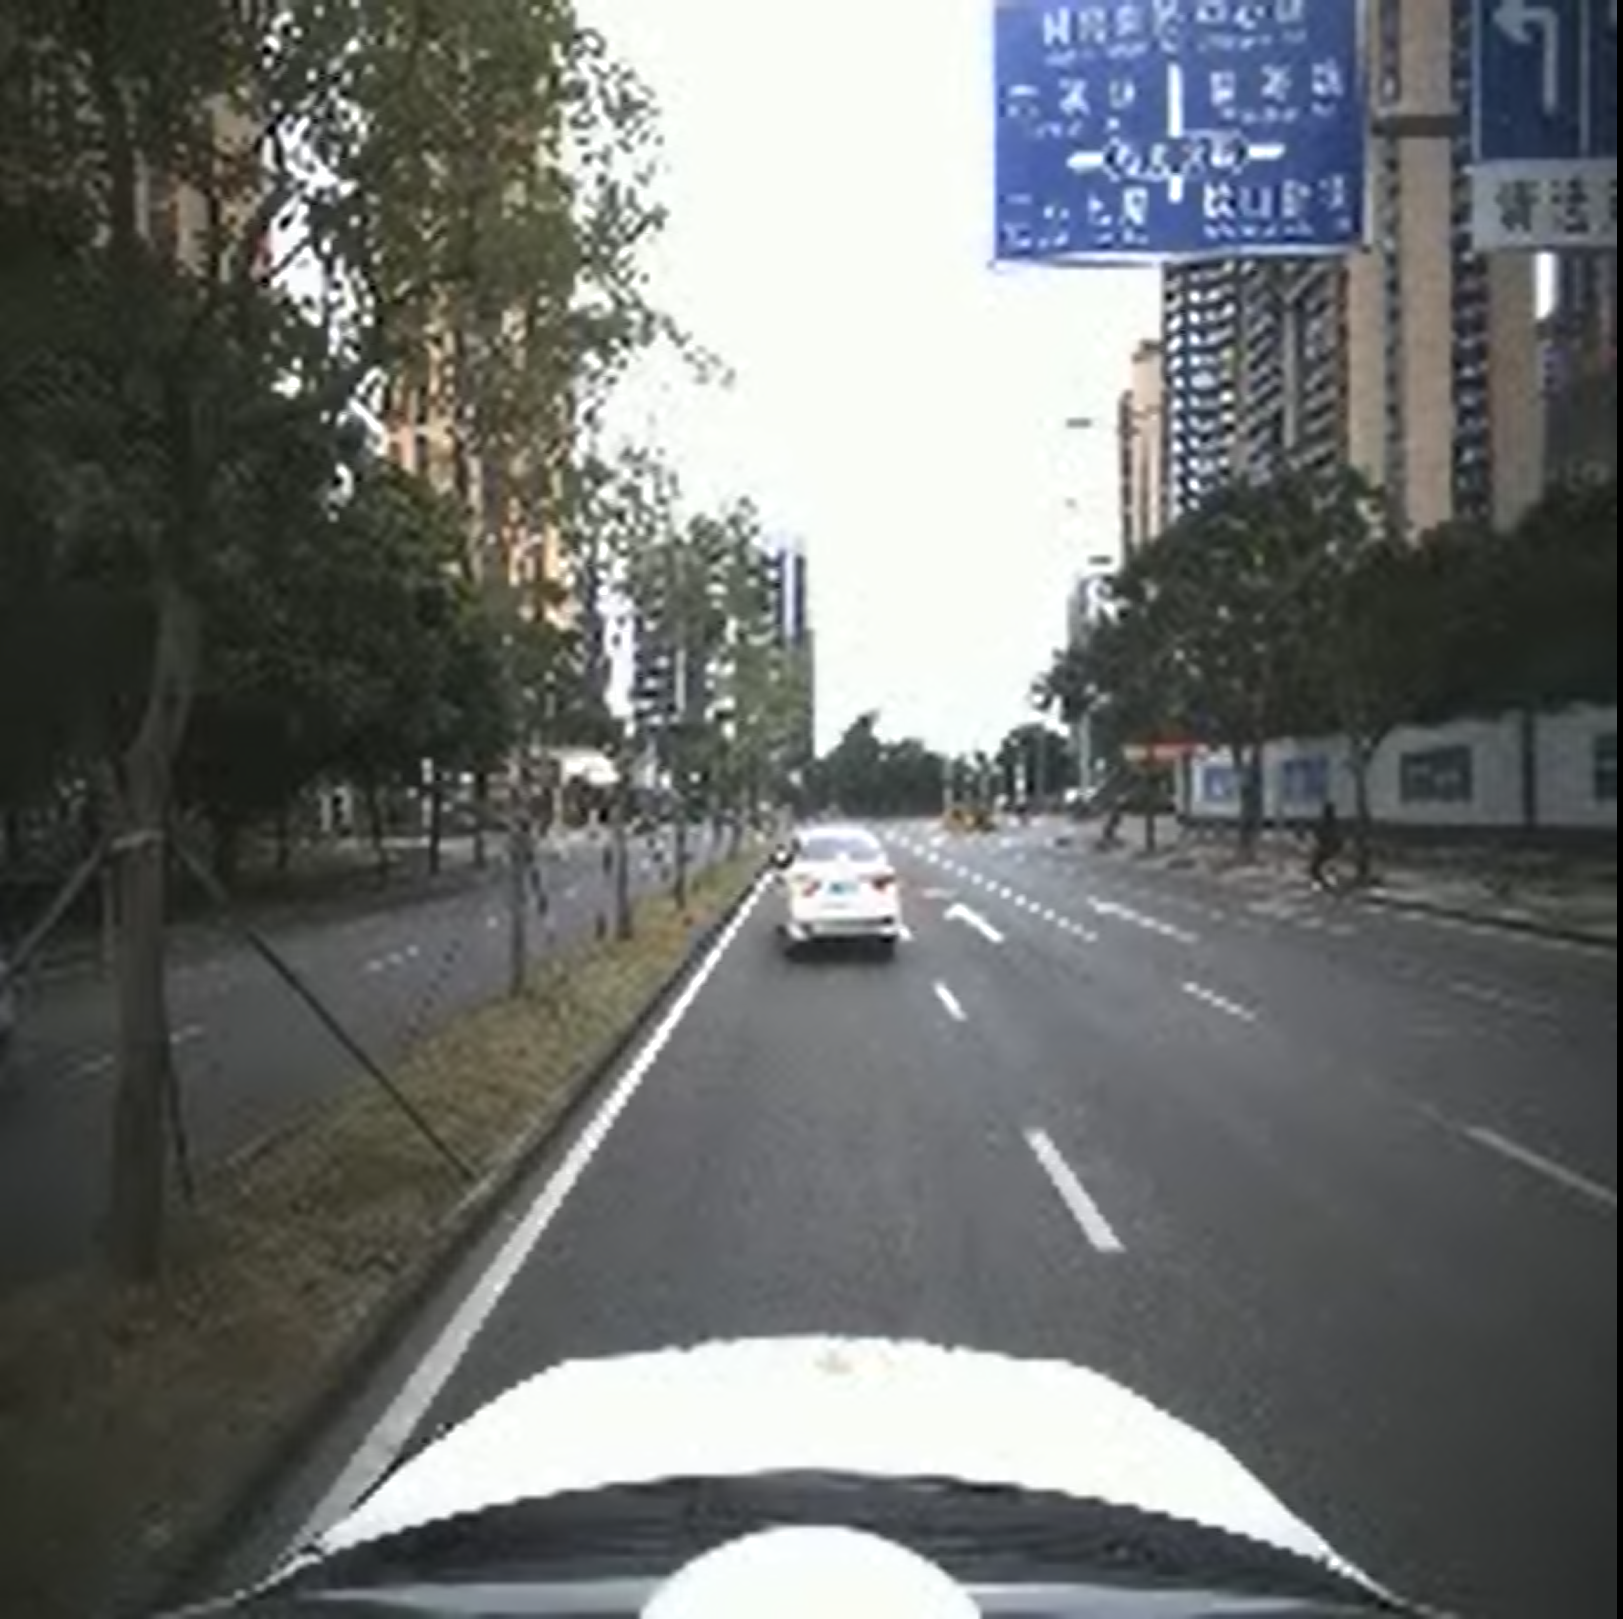
\includegraphics[width=0.20\textwidth]{images/drive_scene4.jpg}
\end{center}

\vspace{0.2em}

% 使用 flushleft 包裹正文内容,保持左对齐
\begin{flushleft}
视频片段与文本标注构成核心数据源:

\begin{itemize}
  \item 数据集命名为 \textbf{Suscape},包含 \textbf{1763 段} 分辨率为 \textbf{224×224} 的前车摄像视频;
  \item 视频时长为 \textbf{2–19 秒},按 \textbf{9:1} 比例划分训练集与验证集;
  \item 文本标注涵盖 \textbf{自车状态与交互信息},用于辅助视频理解与检索建模。
\end{itemize}

\vspace{0.3em}

为探索更优的语义标注方式,我们尝试了\textbf{三种}不同策略:

\begin{itemize}
  \item 三层标签结构;
  \item 语义驱动的人类精修描述;
  \item 自动标注。
\end{itemize}
\end{flushleft}

\end{frame}


\begin{frame}{标注方法一:三层标签结构}

基于早期工作,我们构建了用于自动驾驶场景的\textbf{三层标签结构},用于描述自车状态与周围交互:

\begin{itemize}
  \item 顶层定义\textbf{驾驶行为主类}(如直行、停车等);
  \item 第二层细化为\textbf{具体驾驶策略}(如变道左、变道右);
  \item 第三层刻画\textbf{具体交互语义}(如前车减速、行人穿越)。
\end{itemize}

\vspace{0.4em}

\begin{minipage}[t]{0.48\textwidth}
\textbf{标签结构:}
\begin{flushleft}
\scriptsize\ttfamily
\noindent\texttt{\{}\\
\texttt{ \quad "1.GoStraight": \{}\\
\texttt{ \quad\quad "1.1 InLane": [}\\
\texttt{ \quad\quad\quad "1.1.1 LeadVehicleConstant",}\\
\texttt{ \quad\quad\quad "1.1.2 LeadVehicleDecelerating",}\\
\texttt{ \quad\quad\quad "1.1.3 PedestrianCrossing"}\\
\texttt{ \quad\quad ],}\\
\texttt{ \quad\quad "1.2 ChangingLaneLeft": [],}\\
\texttt{ \quad\quad "1.3 ChangingLaneRight": []}\\
\texttt{ \quad \}}\\
\texttt{\}}
\end{flushleft}
\end{minipage}
\hfill
\begin{minipage}[t]{0.48\textwidth}
\textbf{标注描述示例:}
\begin{flushleft}
\scriptsize\ttfamily
\noindent\texttt{[}\\
\texttt{ \quad \{}\\
\texttt{ \quad\quad "video\_id": "scene-000282-tag-3",}\\
\texttt{ \quad\quad "desc": "The car goes straight in the lane, and the leading vehicle slows down."}\\
\texttt{ \quad \},}\\
\texttt{ \quad \{}\\
\texttt{ \quad\quad "video\_id": "scene-000807-tag-1",}\\
\texttt{ \quad\quad "desc": "The car turns left at the crossroads, and there are no vehicles ahead."}\\
\texttt{ \quad \}}\\
\texttt{]}
\end{flushleft}
\end{minipage}

\end{frame}




\begin{frame}{标注方法一:检索模型性能对比分析}

\textbf{CLIP-ViP 模型下准确度表现(Simple vs DSL):}

\small
\begin{center}
\begin{tabular}{|l|l|c|c|c|c|}
\hline
\textbf{Settings} & \textbf{Direction} & \textbf{Recall@1} & \textbf{Recall@5} & \textbf{Recall@10} & \textbf{Median} \\
\hline
Simple & text-to-video & 5.65\% & 19.77\% & 33.33\% & 22.0 \\
Simple & video-to-text & 1.63\% & 9.11\% & 19.21\% & 27.0 \\
\hline
DSL & text-to-video & 5.65\% & 18.08\% & 30.51\% & 23.0 \\
DSL & video-to-text & 1.63\% & 9.10\% & 19.19\% & 27.0 \\
\hline
\end{tabular}
\end{center}

\vspace{0.2em}
\textbf{精度不足的核心原因:}

\begin{itemize}
  \item \textbf{细节缺失:}  
  同一标签下描述完全相同,但\textbf{视频中的交互行为}差异较大,影响检索准确性。
  
  \item \textbf{覆盖不足:}  
  虽定义多种驾驶场景标签,但仍难以涵盖\textbf{复杂交通交互}情况。

  \item \textbf{语义模糊:}  
  实际场景常涉及\textbf{多标签融合}(如变道+减速+行人穿越),  
  单一标签分类存在边界不清晰,降低标注精度与模型泛化能力。
  
\end{itemize}

\end{frame}

%-------------------------------------------


\begin{frame}{标注方法二:人工标注}

\small
为提升微调性能,我们使用了人工标注策略,相比于之前的三层标签法,人工标注具有以下优势:

\small
\begin{itemize}
  \item \textbf{更全面的交互描述}:覆盖自车状态、前车与邻车动态、障碍物、信号灯与行人行为;
  \item \textbf{相对位置描述更清晰}:如“左侧切入”“右侧切出”明确表达交互方向;
  \item \textbf{减少模糊性与分类歧义}:重点描述与驾驶决策直接相关的信息;
 
\end{itemize}
\normalsize

\textbf{人工标注 标注示例:}

\texttt{\quad "video\_id": "scene-000255-tag-4",}\\
\texttt{\quad "desc": "The car meets a vehicle ahead when changing to the right lane.}\\
\texttt{\quad\quad That vehicle changes to right lane and slows down to stop."}

\end{frame}


\begin{frame}{标注方法二:改进标注方法下的微调性能}

依据改进后的标注原则,我们手动标注了超过 \textbf{1700} 个视频,优化了训练与测试数据;

在 \textbf{CLIP-ViP与VAST} 模型上,微调性能得到显著提升:

\vspace{0.8em}
\textbf{CLIP-ViP 模型下微调性能表现(Simple vs DSL):}

\vspace{0.4em}
\small
\centering
\begin{tabular}{|l|l|c|c|c|c|}
\hline
\textbf{Settings} & \textbf{Direction} & \textbf{Recall@1} & \textbf{Recall@5} & \textbf{Recall@10} & \textbf{Median} \\
\hline
Simple & text-to-video & 14.12\% & 36.16\% & 49.15\% & 11.0 \\
Simple & video-to-text & 4.65\%  & 22.00\% & 40.97\% & 13.0 \\
\hline
DSL    & text-to-video & 14.12\% & 34.46\% & 50.85\% & 10.0 \\
DSL    & video-to-text & 4.63\%  & 22.42\% & 41.28\% & 13.0 \\
\hline
\end{tabular}

\vspace{1.2em}
\begin{minipage}[t]{\textwidth}
\raggedright
\textbf{VAST 数据集微调结果(ITC / ITM 评估指标):}
\end{minipage}

\vspace{0.4em}
\begin{tabular}{|l|l|c|c|c|c|}
\hline
\textbf{Model} & \textbf{Retrieval Direction} & \textbf{Recall@1} & \textbf{Recall@5} & \textbf{Recall@10} & \textbf{Avg} \\
\hline
itc\_tv & text-to-video & 8.5\%  & 35.0\% & 50.3\% & 31.3 \\
itm\_tv & text-to-video & 13.6\% & 42.4\% & 56.5\% & 37.5 \\
\hline
\end{tabular}

\normalsize
\end{frame}






\begin{frame}{标注方法二:人工标注方法下的微调性能(图示)}

对比\textbf{CLIP-ViP模型} \textbf{Simple} 与 \textbf{DSL} 设置下,标注改进前后微调表现:

\centering
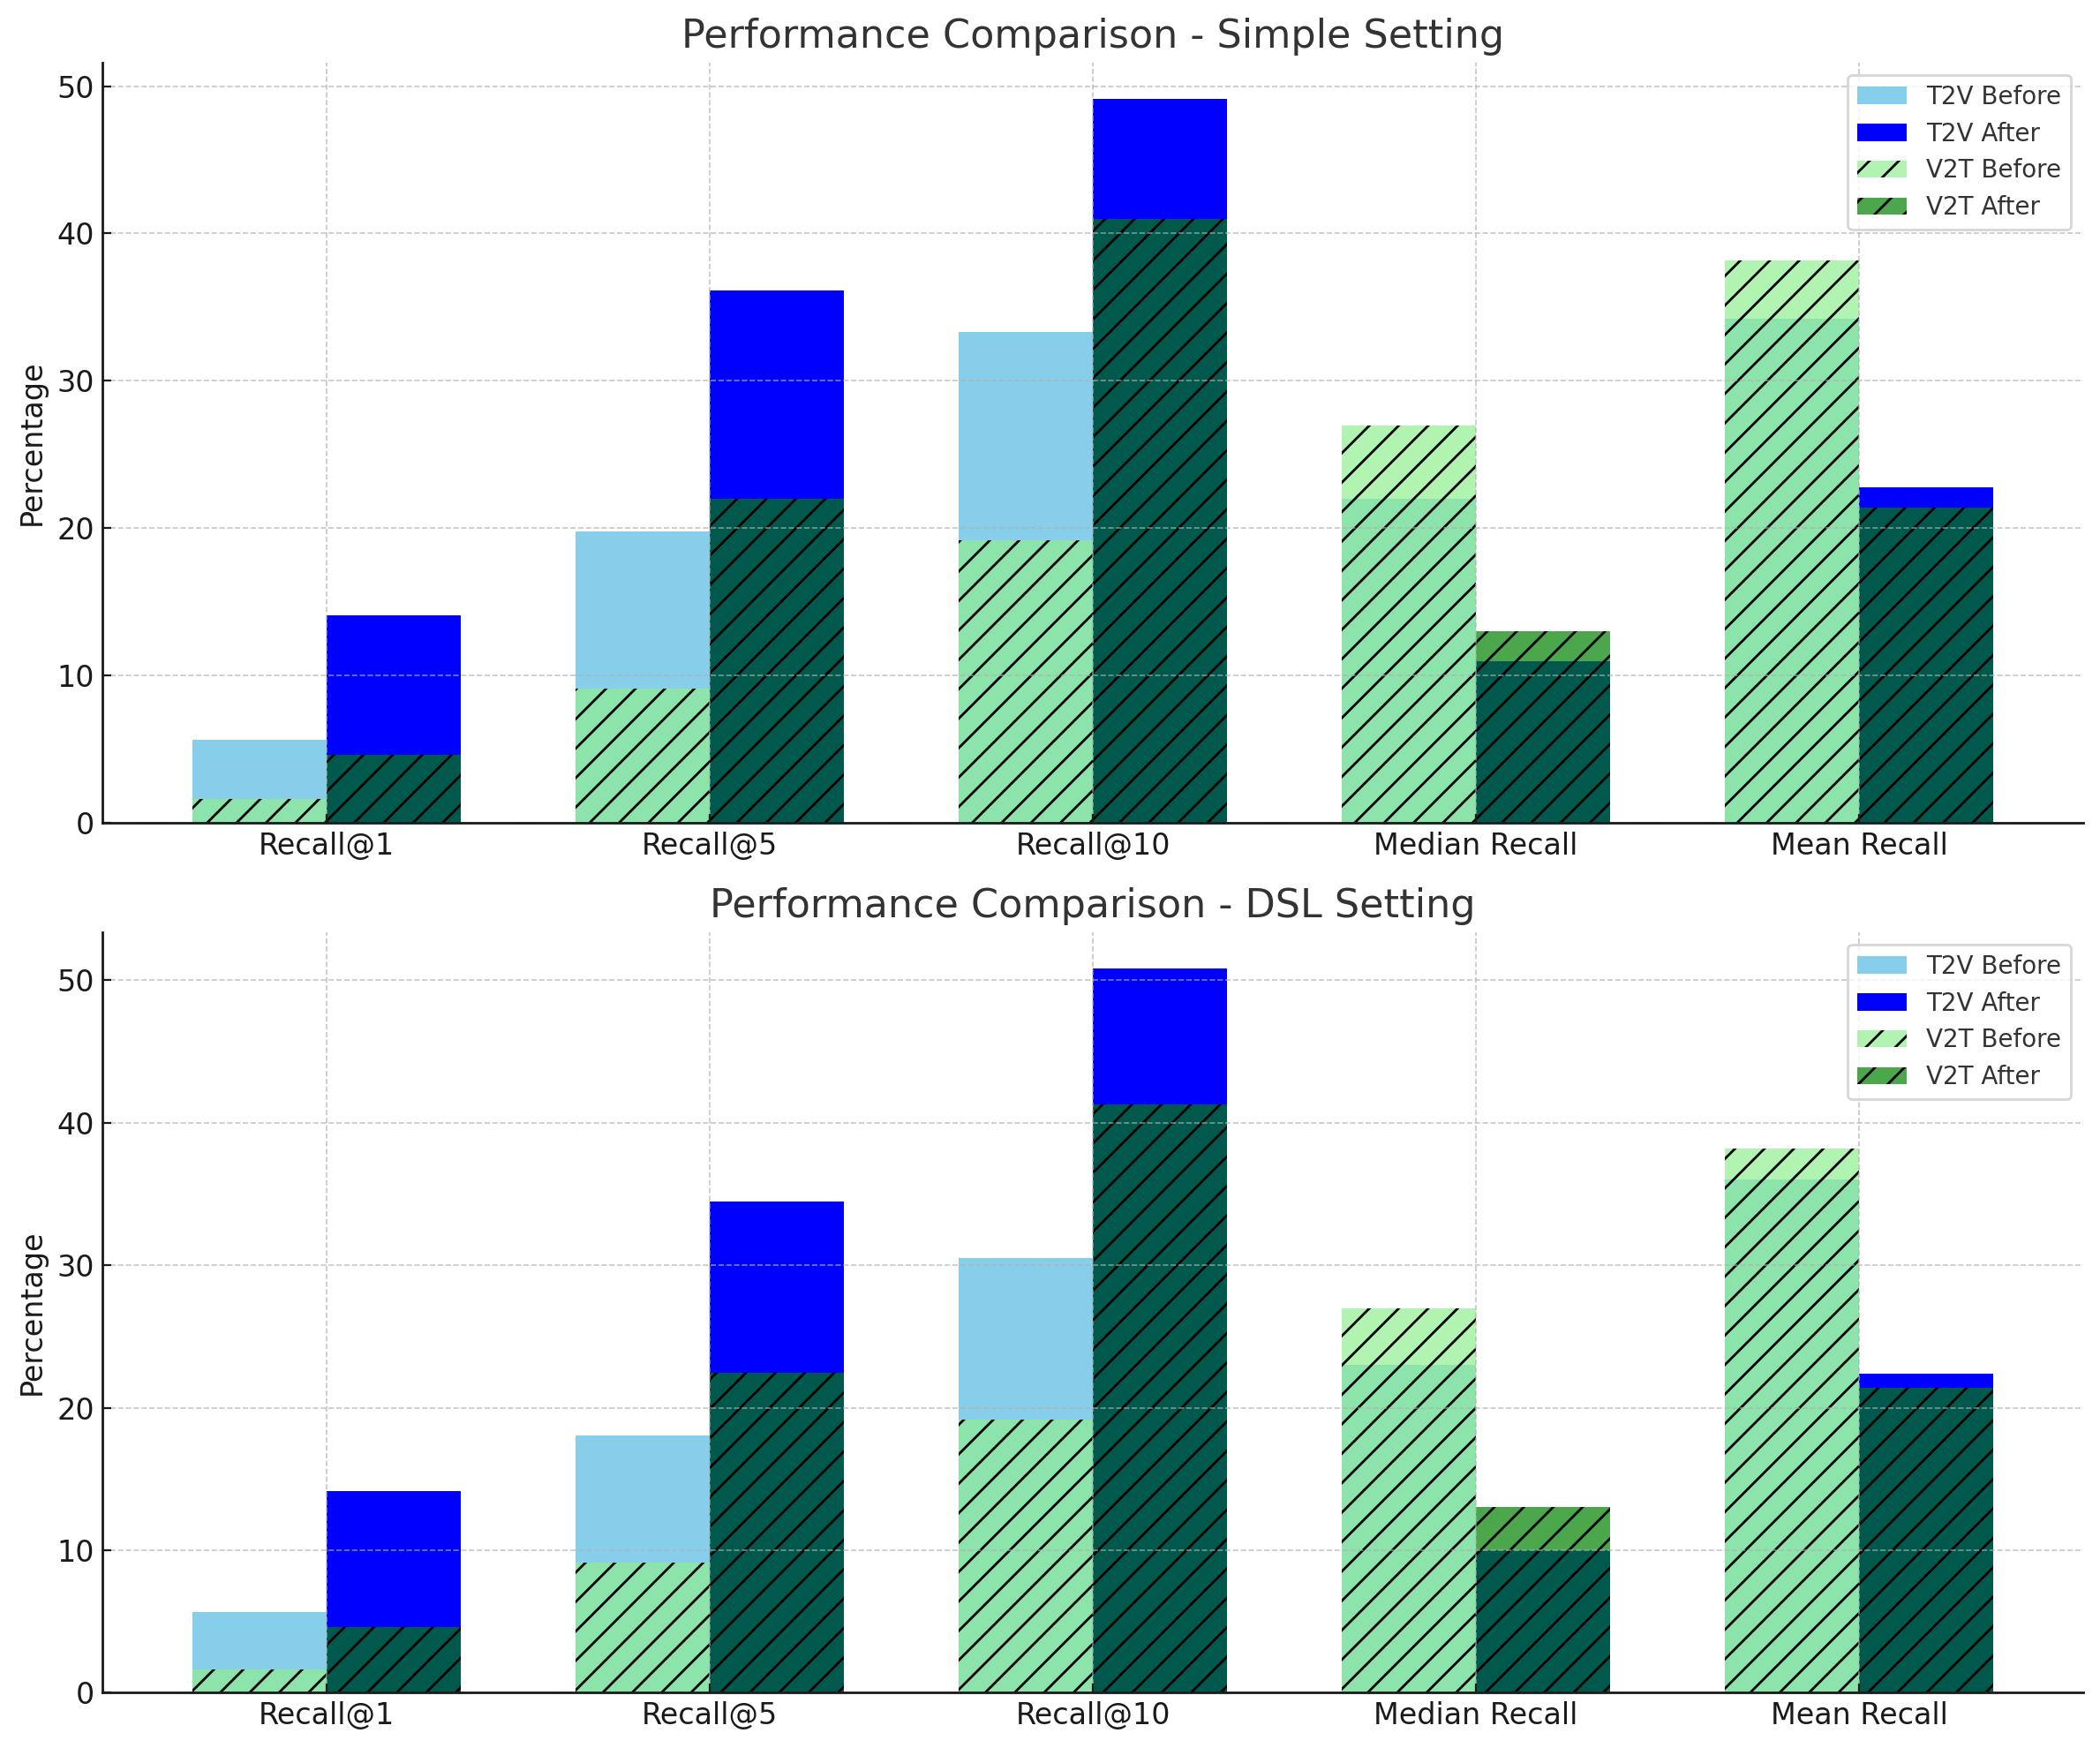
\includegraphics[width=0.72\textwidth]{images/Performance_Comparison_DSL_Setting(HSD).png}

\end{frame}
%------------------------------------------

\begin{frame}{标注方法三:结合 ChatGPT 与关键帧提取的自动字幕生成}

面对手动标注在大数据集上实现困难,我们尝试一种自动化字幕生成策略,结合 \textbf{ChatGPT-4.0} 与 \textbf{关键帧提取},实现对自动驾驶视频的语义生成。

\vspace{0.6em}
\textbf{流程设计:}

\begin{itemize}
  \item 视频划分为 10 个片段,片段 2–9 各随机提取 1 帧;
  \item 片段 1 从后 2/3 采样,片段 10 从前 2/3 采样;
  \item 相邻关键帧时间间隔 $\leq$ 1.5 倍单段时长;
  \item 关键帧按时间排序,作为输入提供给 ChatGPT;
  \item 使用 \texttt{CLIP-ViT-base-patch32} 将图像转为初始文本特征;
  \item ChatGPT 基于上下文与图文提示生成字幕。
\end{itemize}

\textbf{分析:}
\begin{itemize}
\item 提升了自动标注效率
\item 但仍存在一定“幻觉”与时间敏感性不足问题
\end{itemize}

\end{frame}

\begin{frame}{标注方法三:ChatGPT自动字幕生成示例与分析}

\textbf{生成字幕示例:}

\vspace{0.3em}
\texttt{\{"video\_id": "scene-000785-tag-3", "desc": "}The vehicle is driving straight in a lane while \textcolor{red}{overtaking} a slower vehicle in front by \textcolor{red}{changing lanes to the left}, subsequently \textcolor{red}{changing lanes back to the right} in between other vehicles, \textcolor{red}{accelerating} slightly, with frequent interactions, including a vehicle briefly \textcolor{red}{cutting into its lane from the right} before taking off rapidly, and another vehicle \textcolor{red}{overtaking} it from the left, all while approaching a \textcolor{red}{crossroads with a green traffic light}\texttt{"\}}

\vspace{1em}
\textbf{问题:}

\begin{itemize}
  \item 依赖时间顺序的动作(如 \textcolor{red}{加速}/\textcolor{red}{减速})描述仍不准确;
  \item 模型易生成 “合理但虚构” 的 \textcolor{red}{车道切换} 与 \textcolor{red}{交通灯} 内容;
  \item 需要进一步引入视频特征模型,提高对时间依赖行为的识别能力。
\end{itemize}

\end{frame}


\begin{frame}{标注方法三:基于 Video-LLaVA 的自动字幕生成(一)}

\textbf{模型简介:} \texttt{Video-LLaVA} 支持视频 + 文本输入,具备图文联合理解能力(https://github.com/PKU-YuanGroup/Video-LLaVA.git)

\vspace{0.6em}
\textbf{简单提示语:}

\footnotesize
USER: <video> Describe the content of the video in a sentence, and you should focus on the \textcolor{red}{driving status} and the \textcolor{red}{interaction} of the vehicle with other vehicles. The subject of the sentence should be the \textcolor{red}{vehicle}.
\normalsize

\vspace{1em}
\textbf{生成结果示例:}

\texttt{"video\_id": "scene-000783-tag-3"},\\
\texttt{"desc": "A \textcolor{red}{white car} is \textcolor{red}{driving} down a \textcolor{red}{street} with a \textcolor{red}{blue sign} on the side of the road."}

\vspace{0.6em}
\textbf{问题分析:}
\begin{itemize}
  \item 模型聚焦背景信息,忽略驾驶状态与交互;
  \item 难以满足自动驾驶语义标签需求。
\end{itemize}

\end{frame}


\begin{frame}{标注方法三:基于 Video-LLaVA 的自动字幕生成(二)}

\normalsize
\textbf{复杂提示语设计目标:}

\vspace{0.2em}
进一步强调 \textbf{主车行为}、\textbf{车道变化}、\textbf{速度变化}、\textbf{与其他车辆的交互动作}、\textbf{时序特征} 与 \textbf{交通信号}。

\vspace{0.2em}
\textbf{复杂提示语:}

\scriptsize
USER: <video> Describe the content of the video in one sentence, focusing on the \textcolor{red}{vehicle's driving status} and the \textcolor{red}{interactions} with other road users. Include details about its \textcolor{red}{lane positioning}, whether it is driving in a straight lane, changing lanes, turning, merging, or encountering crossroads; whether the vehicle \textcolor{red}{overtakes} others, gets overtaken, or gets \textcolor{red}{cut in}; whether there are \textcolor{red}{speed changes}; and the \textcolor{red}{color of the traffic light}, if present. The subject must be 'the vehicle', and the focus should always be on its behavior and interactions, especially with adjacent vehicles.

\vspace{0.2em}
\normalsize
\textbf{生成结果示例:}

\scriptsize
\texttt{"video\_id": "scene-000785-tag-3"},\\
\texttt{"desc": "The \textcolor{red}{vehicle} is driving straight in a lane while \textcolor{red}{overtaking} a slower vehicle in front by \textcolor{red}{changing lanes} to the left,}\\
\texttt{subsequently changing lanes back to the right in between other vehicles, \textcolor{red}{accelerating} slightly, with frequent interactions,}\\
\texttt{including a vehicle briefly \textcolor{red}{cutting in} from the right, and another vehicle overtaking it from the left,}\\
\texttt{all while approaching a crossroads with a \textcolor{red}{green traffic light}."}

\end{frame}




\begin{frame}{标注方法三:Video-LLaVA自动字幕生成分析}


\textbf{提升:}
\begin{itemize}
  \item 增强了交互和状态细节;
  \item 时间动态信息提取能力提升;
  \item 回答具体问题(如 “车辆是否左转?”、“信号灯颜色?”)时准确率高,说明模型能\textbf{理解局部片段}。
\end{itemize}

\textbf{问题:}

\begin{itemize}
  \item 即便使用复杂提示语,字幕中仍常见 \textbf{背景主导、交互信息缺失} 的问题;
  \item 尝试\textbf{将历史字幕作为“事实提示”}引入提示语,\textbf{但未有效改善生成质量};
  \item 存在一定\textbf{幻觉}(如未出现的 overtaking / cutting 情节);
\end{itemize}

\vspace{0.3em}
\textbf{总结:}
\vspace{0.5em}

\begin{itemize}
  \item 能生成更多车辆行为与交互细节
  \item 生成字幕仍与真实视频存在偏差
  \item 添加提示语可部分提升生成效果
  \item 对时间顺序和动态行为理解有限
\end{itemize}
\end{frame}


%-----------------------------------

\begin{frame}{标注方法三:基于 Video-LLaMA2 的自动字幕生成}

\scriptsize

\textbf{模型简介:} \texttt{Video-LLaMA2} 模型在 CoVLA 数据集字幕生成任务中表现出色,故我们决定尝试该模型。\\
\texttt{https://github.com/DAMO-NLP-SG/VideoLLaMA2.git}

\vspace{0.3em}
\textbf{提示语设计:}给定已有的简单二级标签+通用复杂prompt

\texttt{instruct = 'You should remember that the information ' + truth + " is a truth. Describe the content of the video and you must according to the truth to adjust your answer. You should focus on the \textcolor{red}{driving status} of the ego vehicle itself and the \textcolor{red}{driving status} of the leading vehicle, the \textcolor{red}{interactions} with other road users in detail, and add any other \textcolor{red}{factors} that may affect the driving of the ego vehicle to make your answer cover more \textcolor{red}{aspects} that are not given by the truth but appear in the video. You should summarize your answer to make it concise and avoid the description about the background scenery such as buildings and trees."}

\vspace{0.3em}
\textbf{生成字幕示例:}

\texttt{"video\_id": "scene-000783-tag-3"},\\
\texttt{"desc": "The video shows a car \textcolor{red}{driving} down an  \textcolor{red}{empty street}. The car \textcolor{red}{maintains its lane} and continues straight ahead \textcolor{red}{without} any obstacles or other vehicles in sight. The road appears to be well-maintained with clear markings and \textcolor{red}{no} signs of \textcolor{red}{traffic} or \textcolor{red}{congestion}. The car's \textcolor{red}{speed} is consistent throughout the video, indicating that it is \textcolor{red}{driving at a steady pace}. There are \textcolor{red}{no pedestrians} or \textcolor{red}{cyclists} visible on the street, and the surrounding area appears to be quiet and peaceful. Overall, the video depicts a smooth and uneventful drive down an empty street."}

\normalsize

\end{frame}

\begin{frame}{标注方法三:Video-LLaMA2 自动字幕生成分析}

使用Video-LLaMA2自动生成的字幕,在 \textbf{CLIP-ViP} 和 \textbf{VAST} 模型上进行了文本到视频的检索任务评估

\vspace{0.4em}
\textbf{CLIP-ViP 模型评估结果:}

\vspace{0.5em} 
\normalsize
\scriptsize
\centering
\begin{tabular}{|l|l|c|c|c|c|c|}
\hline
\textbf{Settings} & \textbf{Direction} & \textbf{Recall@1} & \textbf{Recall@5} & \textbf{Recall@10} & \textbf{Median Recall} & \textbf{Mean} \\
\hline
Simple & text-to-video   & 24.86\% & 57.06\% & 69.49\% & 4.0 & 12.2 \\
Simple & video-to-text   & 26.08\% & 50.54\% & 69.02\% & 5.0 & 12.2 \\
\hline
DSL    & text-to-video   & 27.68\% & 57.06\% & 72.88\% & 4.0 & 12.4 \\
DSL    & video-to-text   & 26.08\% & 50.54\% & 69.02\% & 5.0 & 12.3 \\
\hline
\end{tabular}

\vspace{0.5em} % 减少此处的间距
\raggedright
\textbf{\normalsize VAST 模型评估结果:} % 改为raggedright以减小与表格的间距

\vspace{0.3em} 
\normalsize
\begin{center}
\begin{tabular}{|l|l|c|c|c|c|}
\hline
\textbf{Model} & \textbf{Direction} & \textbf{Recall@1} & \textbf{Recall@5} & \textbf{Recall@10} & \textbf{Avg} \\
\hline
itc\_tv & text-to-video & 23.7\% & 56.5\% & 73.4\% & 51.2 \\
itm\_tv & text-to-video & 31.1\% & 65.0\% & 80.2\% & 58.8 \\
\hline
\end{tabular}
\end{center}

\end{frame}



\begin{frame}{标注方法三:Video-LLaMA2 自动字幕生成分析}

\begin{minipage}[t]{0.48\textwidth}
  \centering
  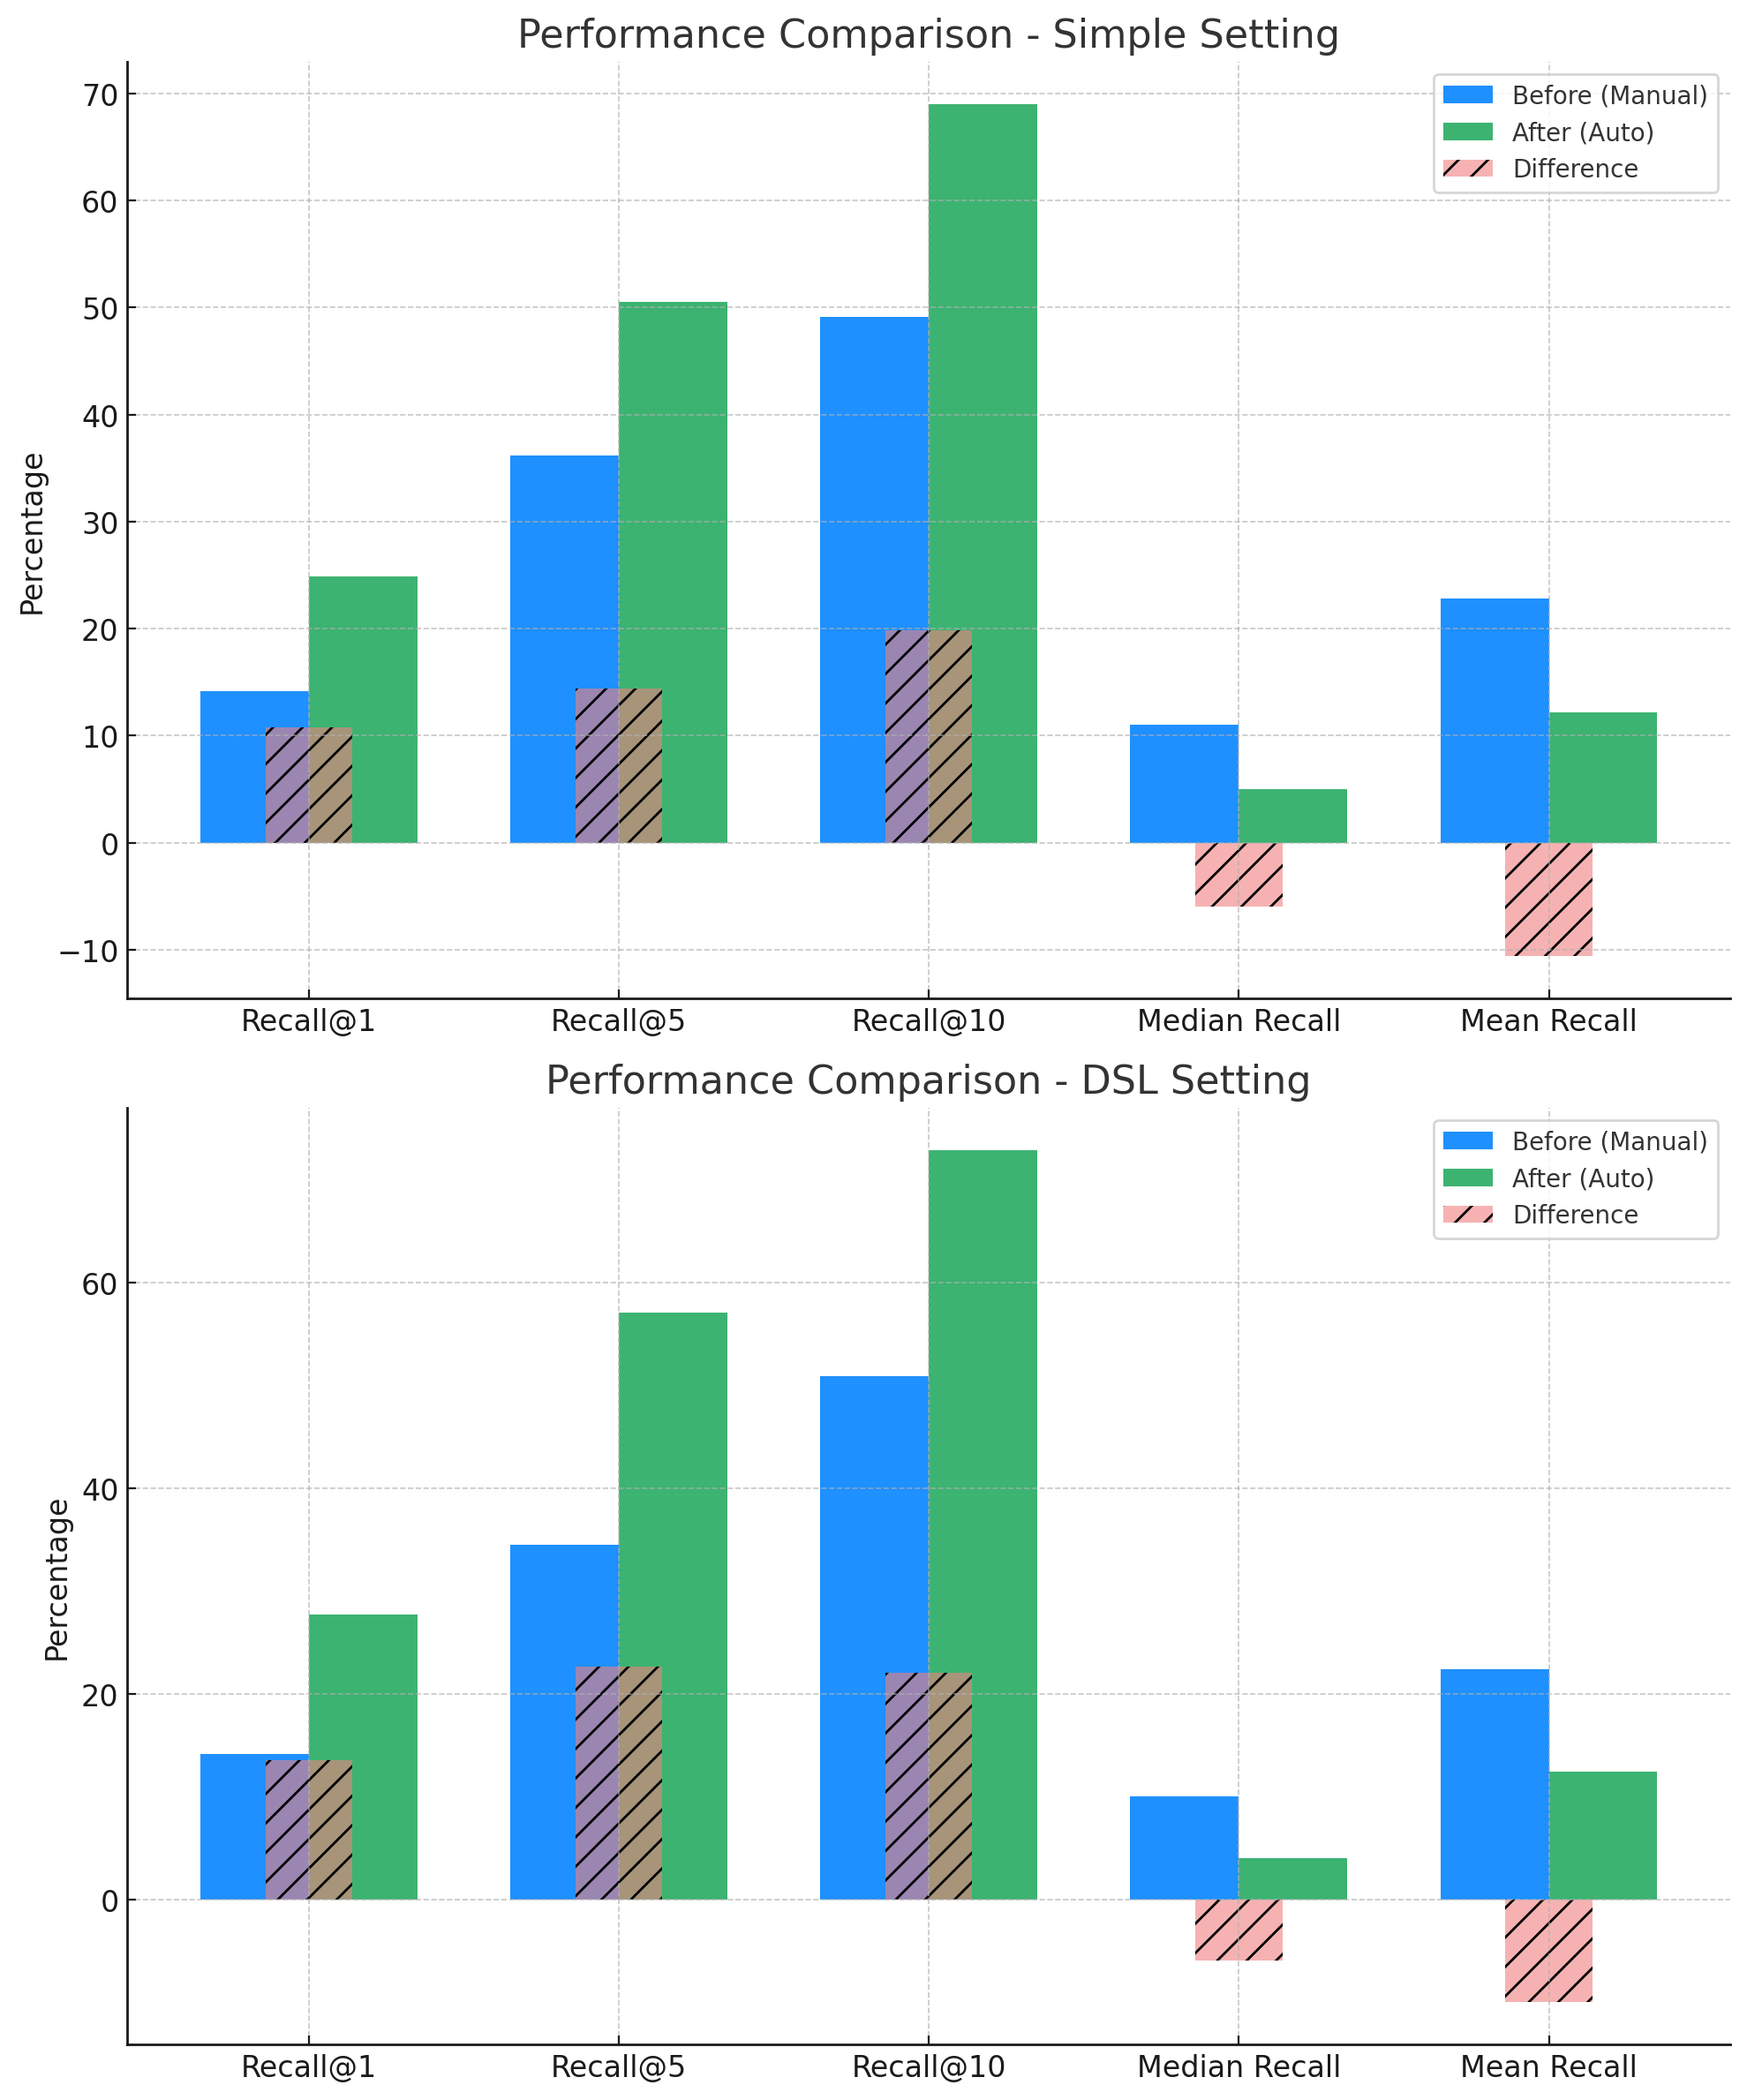
\includegraphics[width=0.95\linewidth]{images/performance comparison between manual and auto on CLIP-VIP.png}
  \vspace{0.1em}
  \textbf{\small CLIP-ViP 检索性能}
\end{minipage}
\hfill
\begin{minipage}[t]{0.48\textwidth}
  \centering
  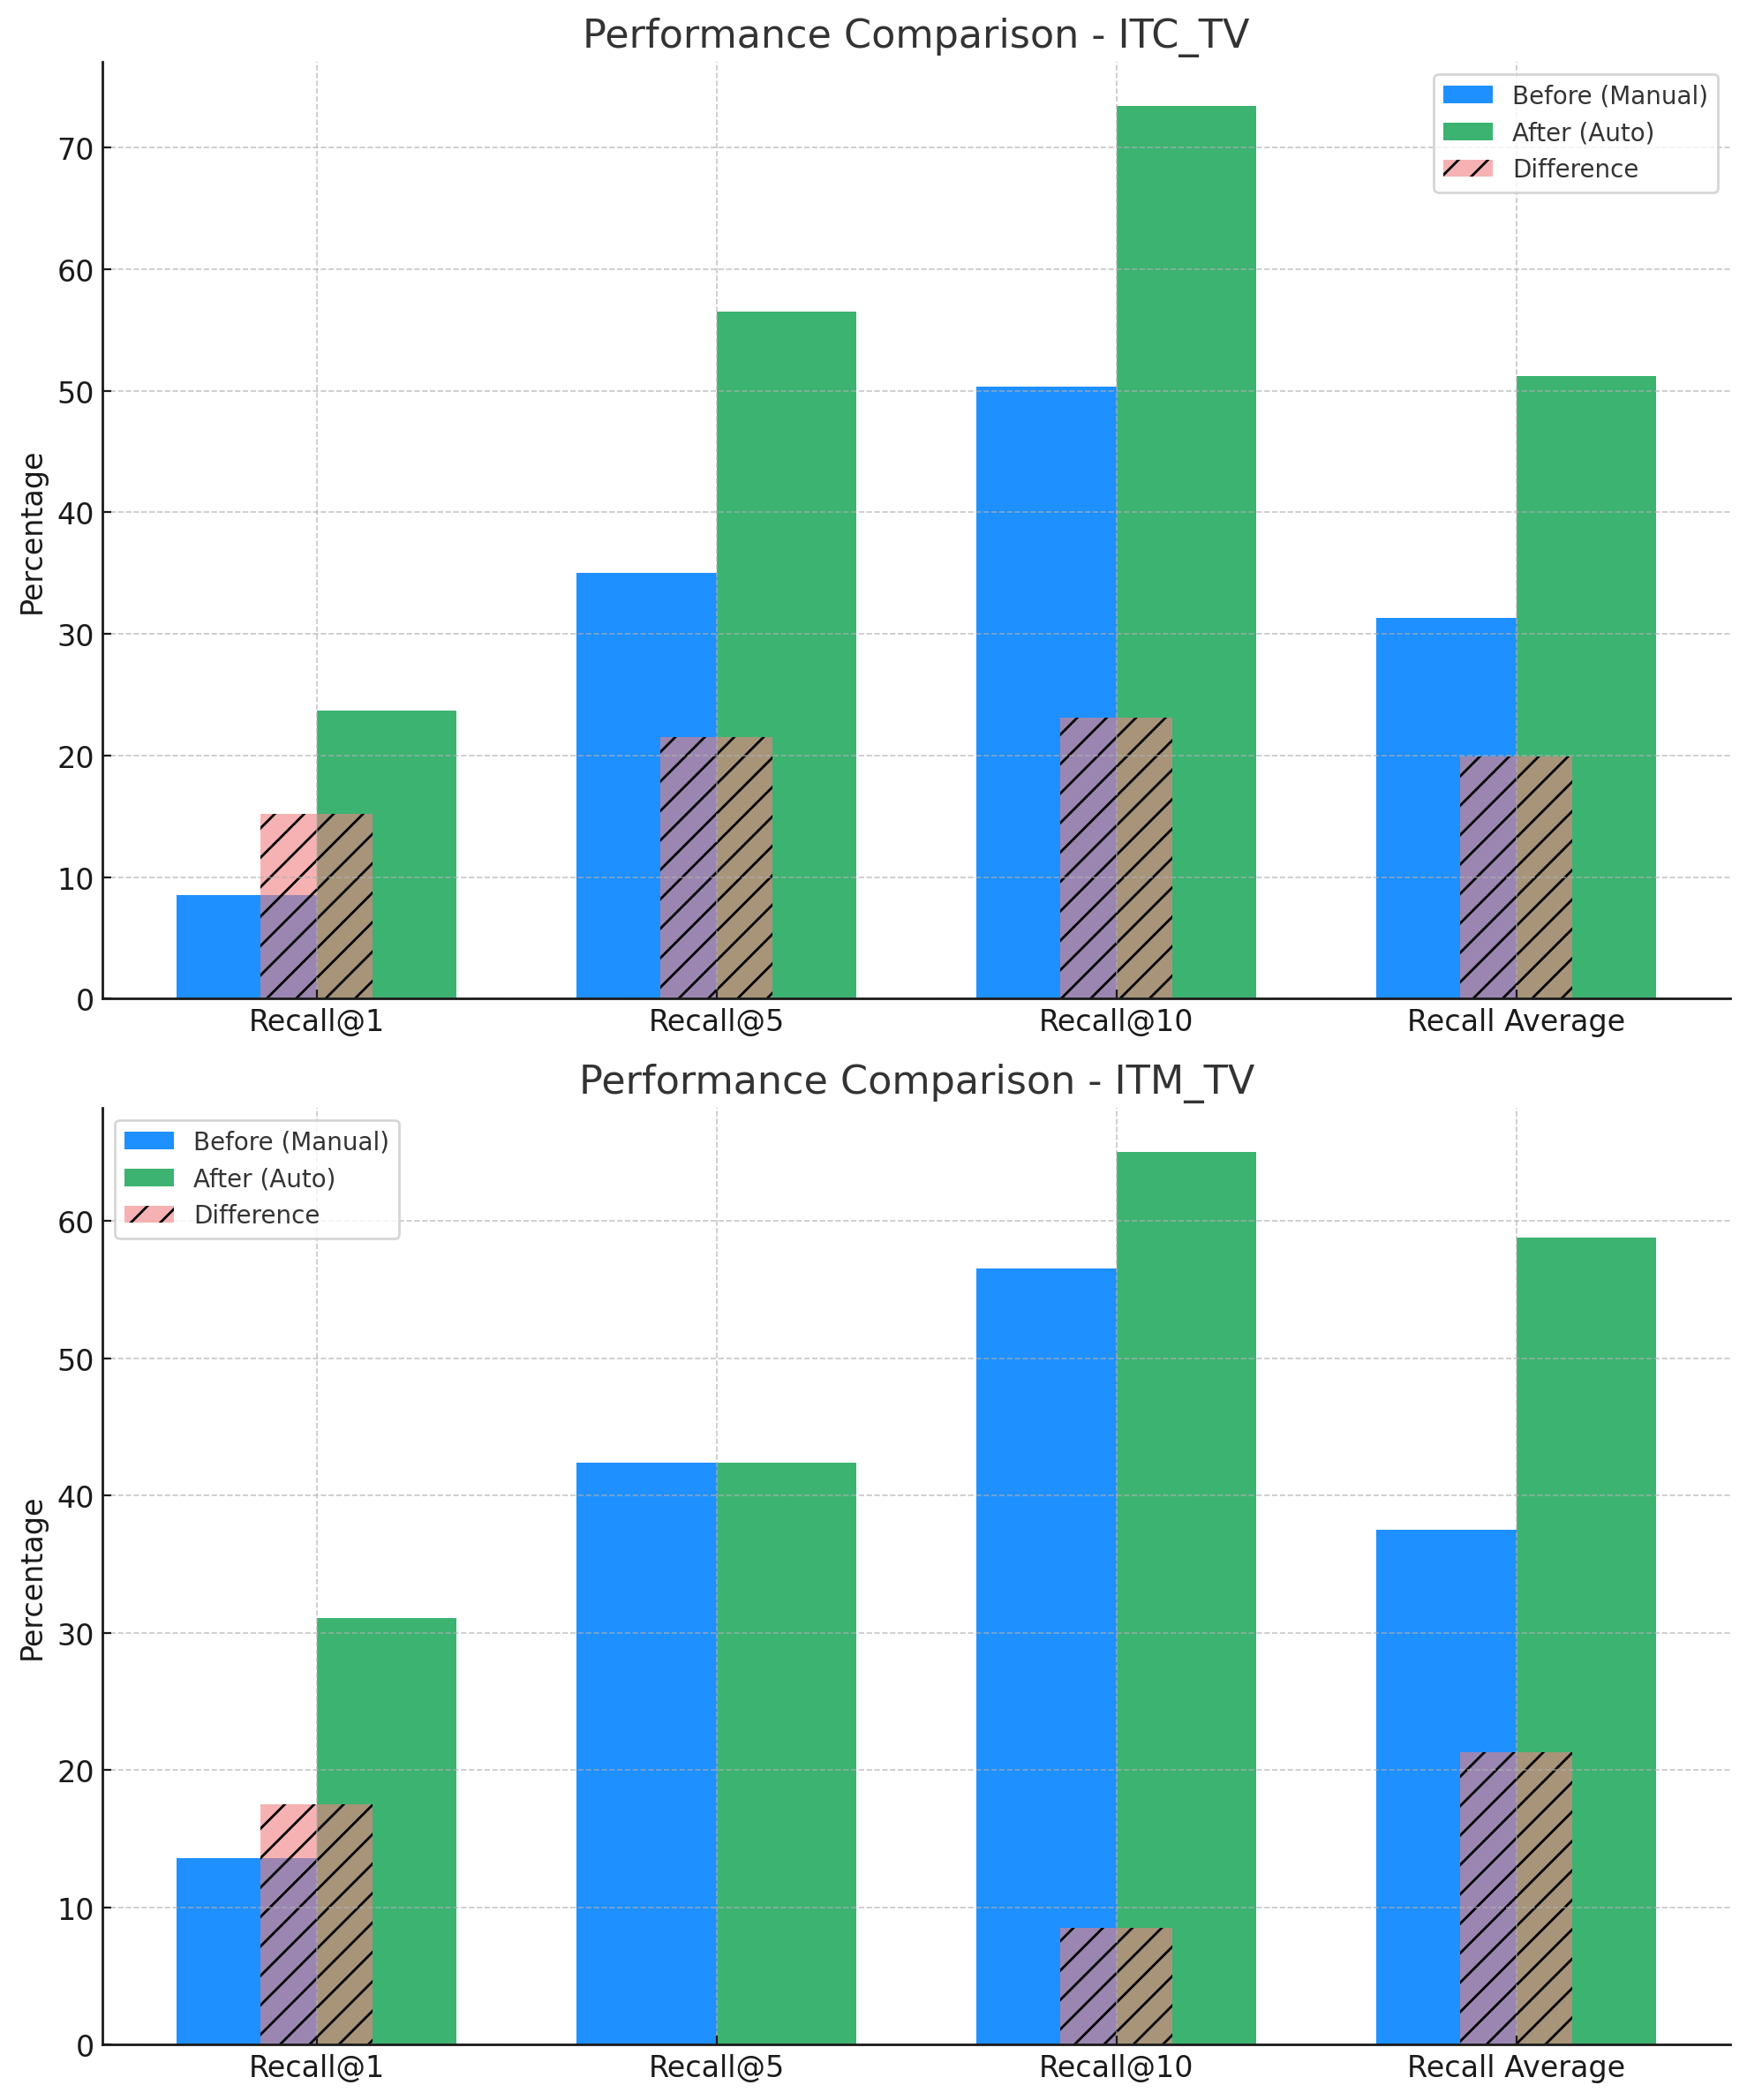
\includegraphics[width=0.95\linewidth]{images/performance camparison bewteen manual and auto on VAST.png}
  \vspace{0.1em}
  \textbf{\small VAST 检索性能}
\end{minipage}

\vspace{0.2em}

\footnotesize
\textbf{总结:} Video-LLaMA2 自动字幕在两模型上的评估结果,均显著优于手动标注,具备更高质量、更多交互细节、更强泛化性,且人工成本更低
\normalsize

\end{frame}

%-------------------------------

\section{多轮问答设计与模型推理}

\begin{frame}{多轮问答设计理念}
  \begin{itemize}
    \item \textbf{实现操作}
    \begin{itemize}
      \item 通过\textbf{多轮交互式问答},逐步细化视频场景的\textbf{标签内容}
      \item 利用已有的\textbf{二级标签}作为前提,指导模型生成更精确的\textbf{三级标签描述}
      \item 设计多种\textbf{问答方式},验证不同策略对生成效果的影响
    \end{itemize}

    \vspace{1em}

    \item \textbf{可行性分析}
    \begin{itemize}
      \item \textbf{VideoLLaMA2}等先进模型已结合二级标签信息辅助生成,验证基于标签的\textbf{辅助推理}有效性
      \item 相关论文(DriveLM)显示,\textbf{思维链(Chain-of-Thought)推理}显著提升大语言模型的复杂任务表现与准确率
    \end{itemize}
  \end{itemize}
\end{frame}

\begin{frame}{第一种问答设置}
\textbf{提问设计特点:}
\begin{itemize}
  \item 采用\textbf{固定且简洁的问题列表},覆盖车辆周边基础交互信息;但未细化标签定义
  \item 问题围绕\textbf{前车位置、交通信号、障碍物、车辆切入/切出、行人穿越、车辆状态}等核心场景要素
  \item 最后以选择题形式确定\textbf{对应的三级标签}
\end{itemize}

\vspace{0.6em}
\textbf{完整问题列表示例:}

\footnotesize
\begin{itemize}
  \item Is there a leading vehicle ahead driving in the same lane as the ego vehicle?
  \item Is there a traffic light ahead?
  \item Are there obstacles ahead?
  \item What is the shape of the traffic light? Round or Arrow.
  \item Are there vehicles cutting in or cutting out of the lane ahead?
  \item Does the leading vehicle stop?
  \item Are there vehicles crossing the road ahead?
  \item Is there pedestrian crossing the road?
  \item Which label fits the video best, LeadVehicleCutOut, VehicleCutInAhead, LeadVehicleStopped, LeadVehicleWrongDriveway or PedestrianCrossing?
\end{itemize}
\normalsize

\end{frame}

\begin{frame}{第一种问答结果}

\begin{figure}
    \centering
    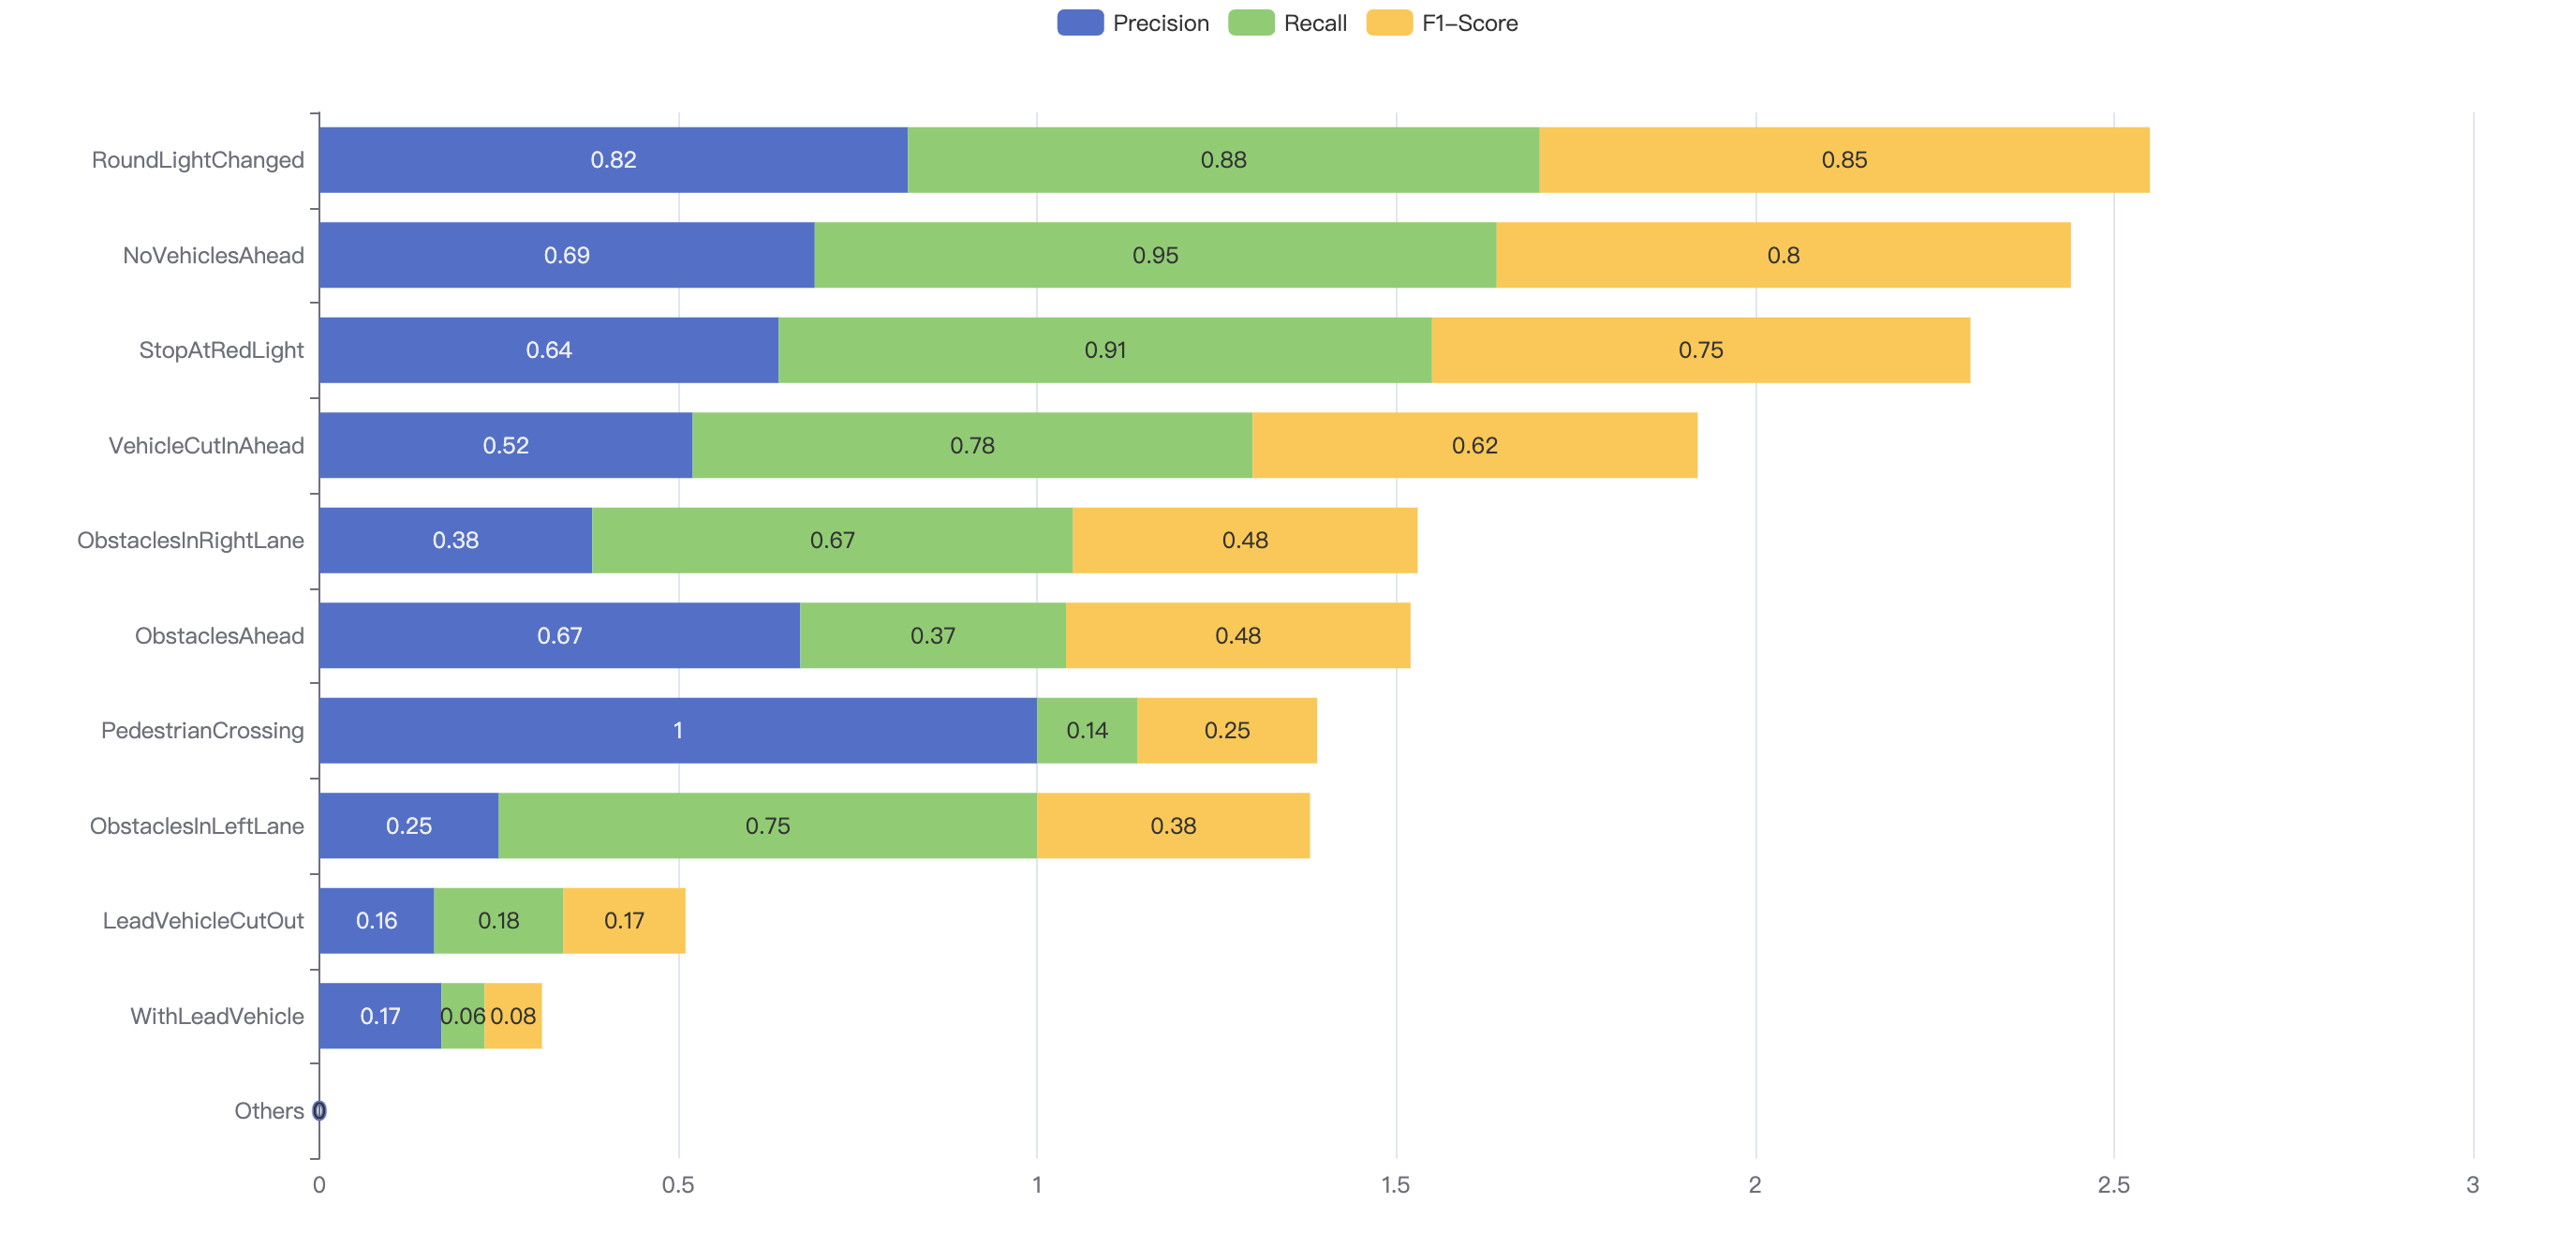
\includegraphics[width=1\linewidth]{images/result1.png}
    \caption{第一种问答生成三级标签的结果}
\end{figure}

\scriptsize
Others:LeadVehicleStopped, StopAtGreenLight, StopAtYellowLight, RidingLane, ArrowLightChanged, StopAtFlashGreenLight, VehiclesCrossing, LeadVehicleStppoed, LeadVehicleWrongDriveway    
\normalsize
\end{frame}


\begin{frame}{第一种问答:错误分析}

\begin{minipage}[t]{0.4\textwidth}
  \centering
  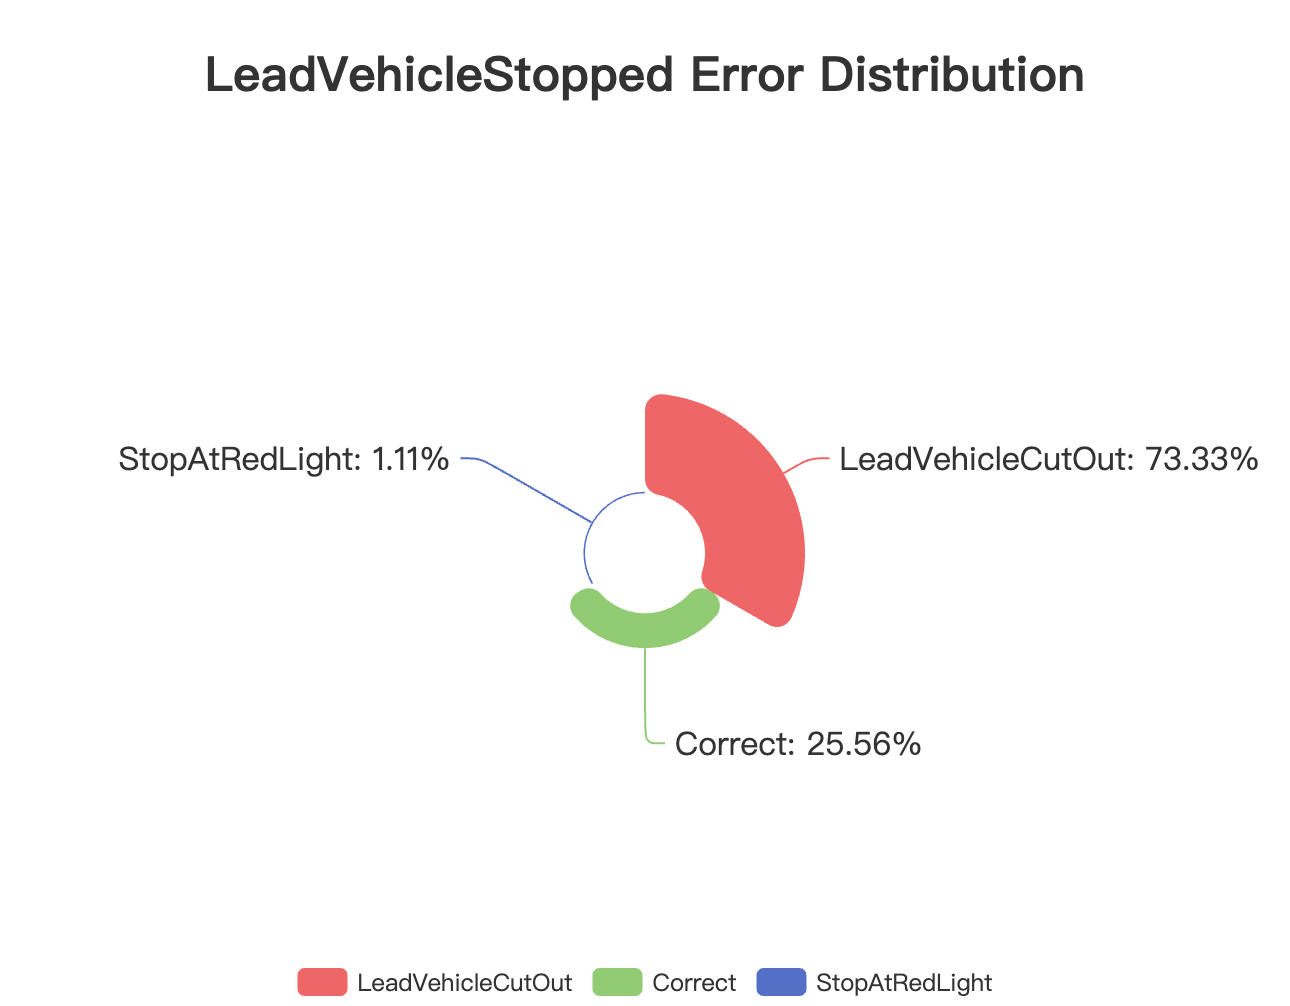
\includegraphics[width=\linewidth]{images/Q1 LeadVehicleStopped Error Distribution.png}
\end{minipage}
\hfill
\begin{minipage}[t]{0.4\textwidth}
  \centering
  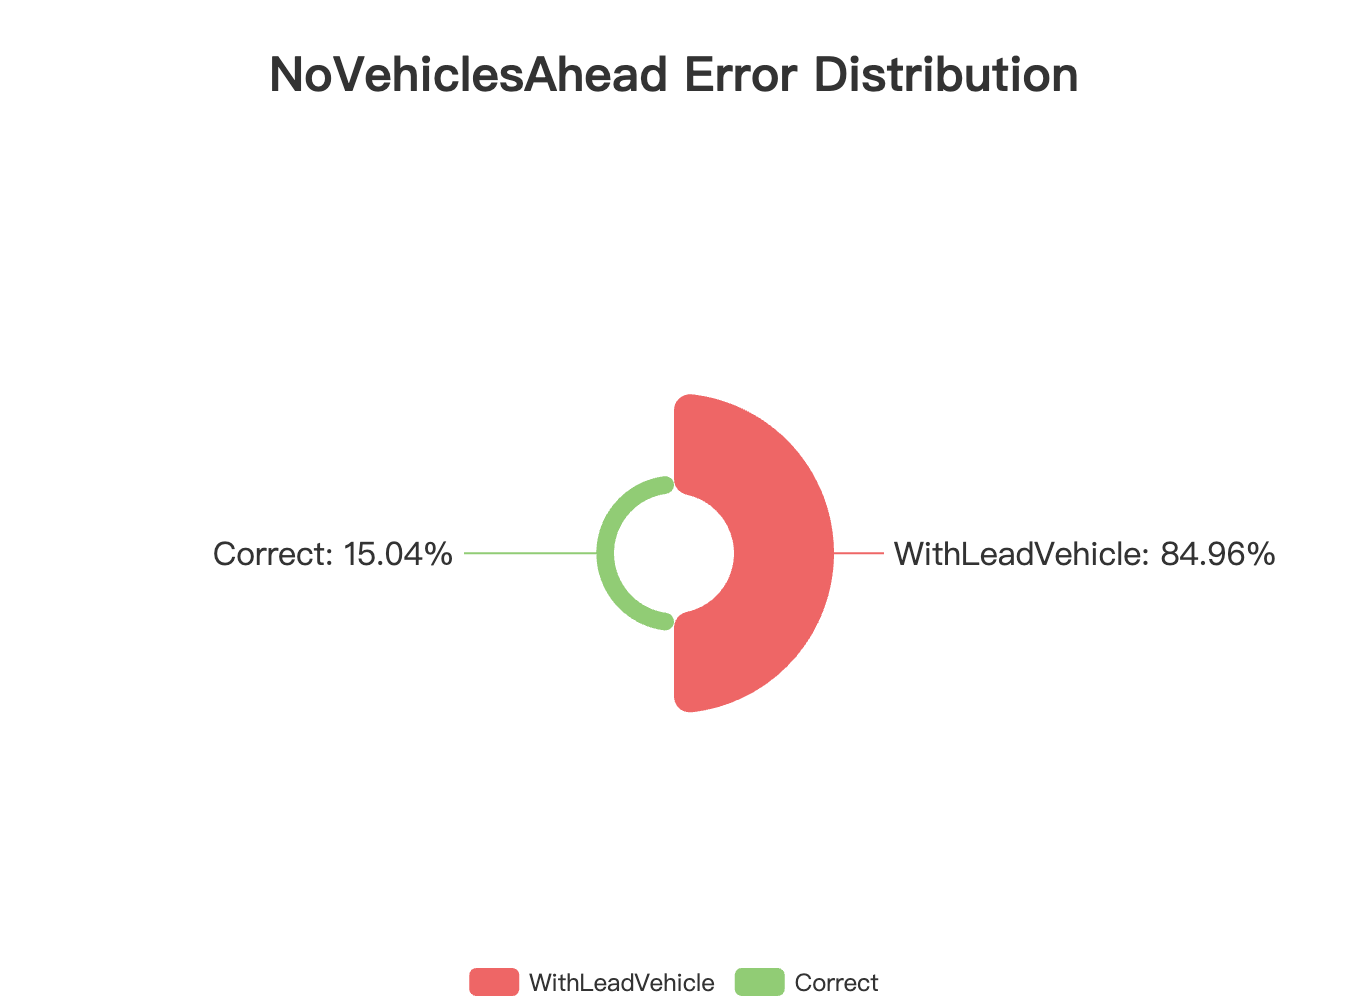
\includegraphics[width=\linewidth]{images/Q1 NoVehiclesAhead Error Distribution.png}
\end{minipage}


\begin{minipage}[t]{0.4\textwidth}
  \centering
  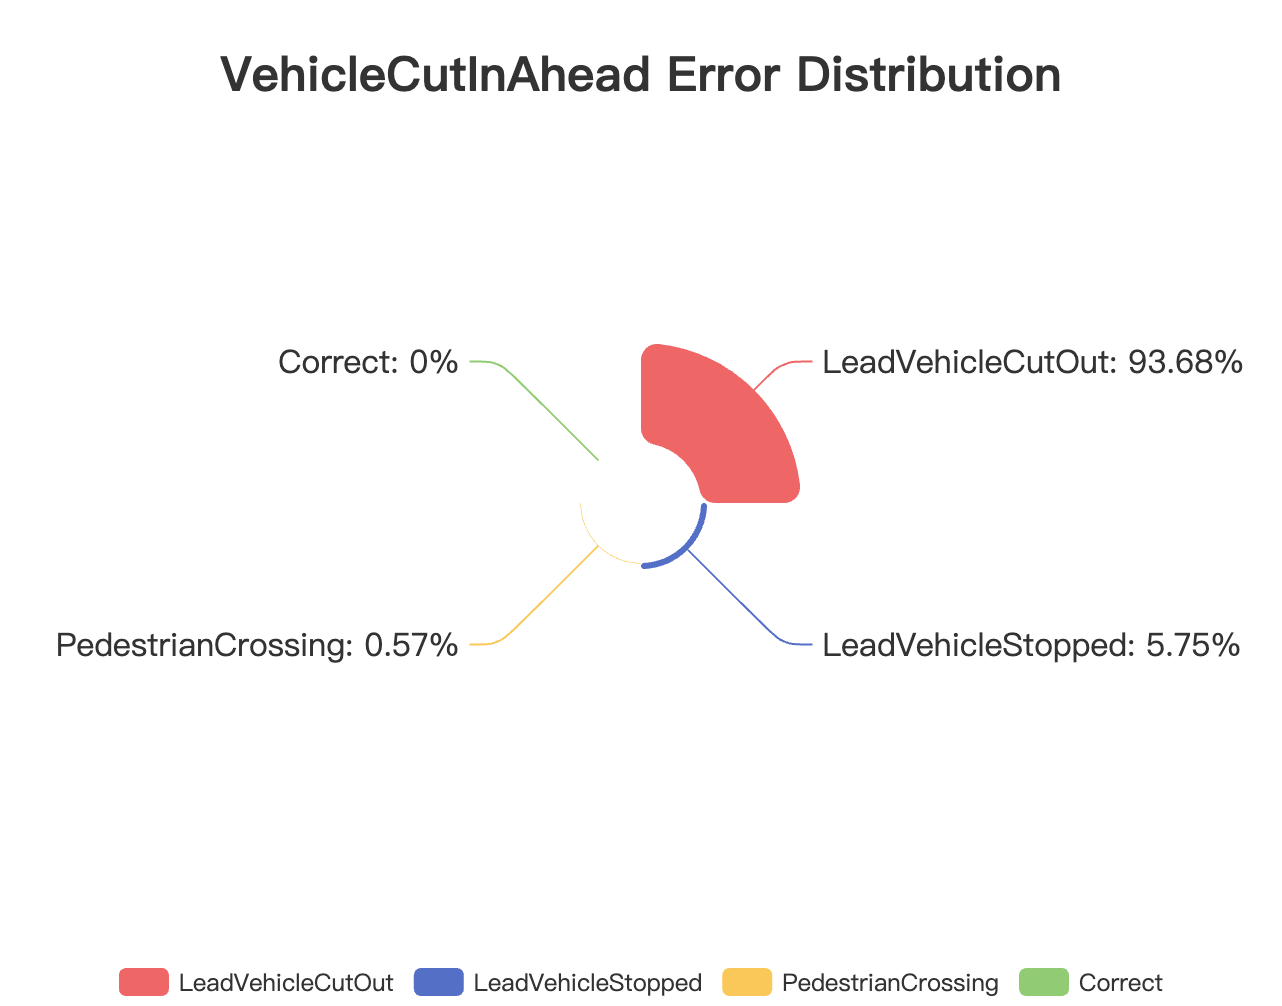
\includegraphics[width=\linewidth]{images/Q1 VehicleCutInAhead Error Distribution.png}
\end{minipage}
\hfill
\begin{minipage}[t]{0.4\textwidth}
  \centering
  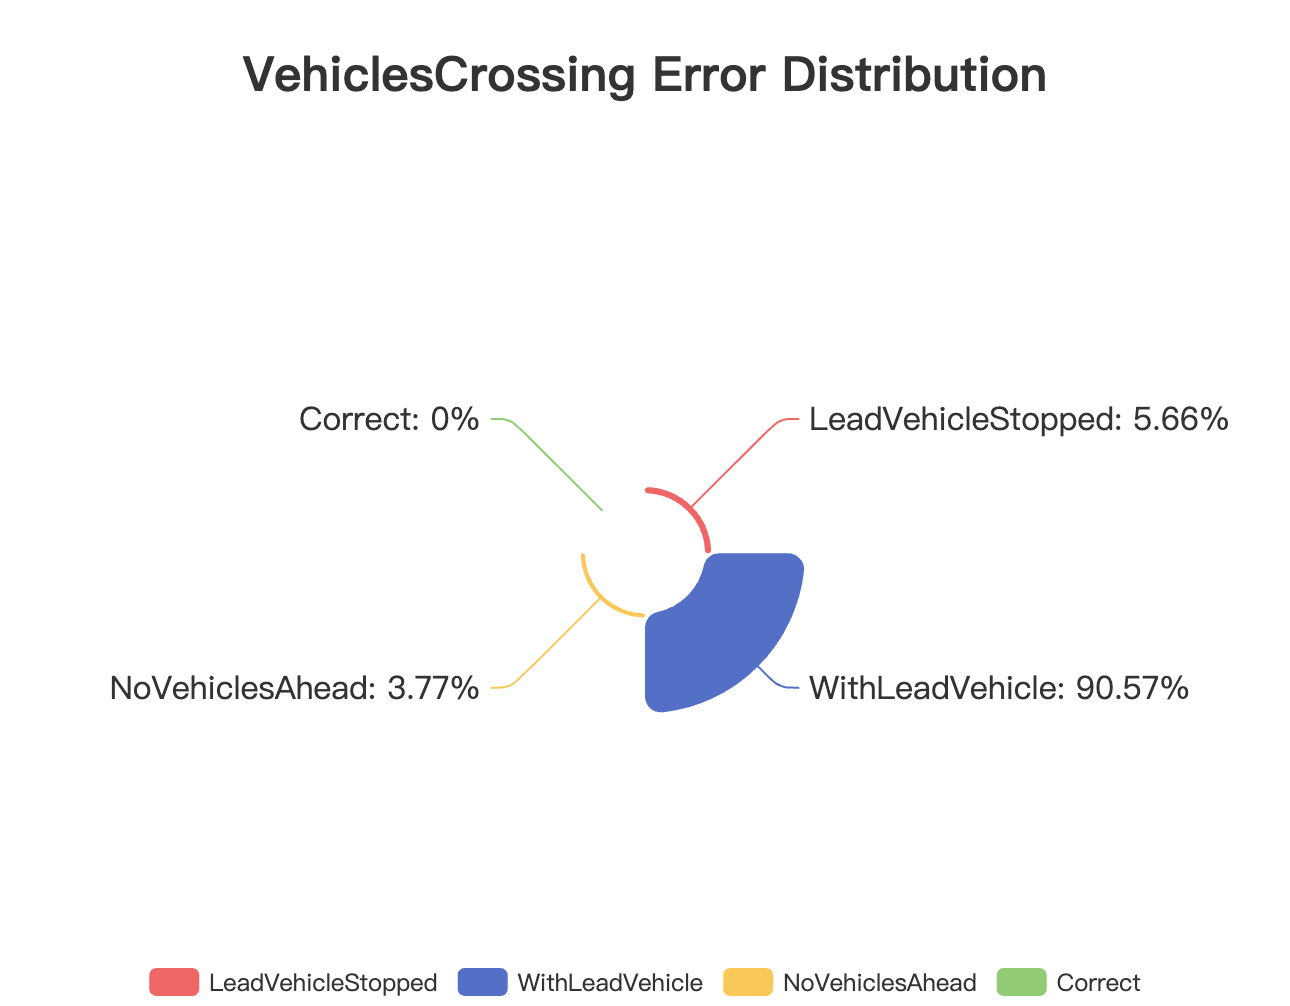
\includegraphics[width=\linewidth]{images/Q1 VehiclesCrossing Error Distribution.png}
\end{minipage}


\end{frame}


\begin{frame}{第二种问答设置(上)}
\scriptsize
\textbf{提问设计特点:}
\begin{itemize}
  \item 问题增加了对\textbf{三级标签定义}的明确说明,使模型理解更具体全面
  \item 采用\textbf{多步骤思维链式提问},层层引导模型细化判断
  \item 涉及\textbf{车辆切入切出}、\textbf{停止}、\textbf{逆行}、\textbf{交通信号}、\textbf{障碍物}、\textbf{行人}、\textbf{驾驶轨迹}等多维度信息
\end{itemize}

\vspace{0.6em}
\textbf{完整问题列表示例(1):}

\begin{itemize}
  \item Is there a \textcolor{red}{leading vehicle} in the \textcolor{red}{current lane} \textcolor{red}{ahead}? A leading vehicle means a vehicle or a motorcycle \textcolor{red}{driving} in the front exactly in the \textcolor{red}{same lane} as the ego vehicle or a vehicle \textcolor{red}{driving} in front of and in the same direction as the ego vehicle when \textcolor{red}{crossing}.
  \item Is there a \textcolor{red}{leading vehicle} or a \textcolor{red}{leading motorcycle} \textcolor{red}{cutting into} the lane of the ego vehicle? \textcolor{red}{Cutting in} means the leading vehicle \textcolor{red}{enters} the lane of the ego vehicle from the \textcolor{red}{adjacent} lane \textcolor{red}{ahead}.
  \item Is there a \textcolor{red}{leading vehicle} or a \textcolor{red}{leading motorcycle} \textcolor{red}{cutting out} of the lane of the ego vehicle? \textcolor{red}{Cutting out} means the leading vehicle \textcolor{red}{leaves} from the lane of the ego vehicle to the \textcolor{red}{adjacent} lane \textcolor{red}{ahead}.
  \item Does the \textcolor{red}{leading vehicle} \textcolor{red}{stop}?
  \item Is there a \textcolor{red}{traffic light} \textcolor{red}{ahead}? What is the \textcolor{red}{shape}, round or arrow?
  \item Does the \textcolor{red}{ego vehicle} \textcolor{red}{stop}? If so, why does the ego vehicle stop?
\end{itemize}
\normalsize
\end{frame}


\begin{frame}{第二种问答设置(下)}
\scriptsize
\textbf{提问设计特点:}
\begin{itemize}
  \item 问题增加了对\textbf{三级标签定义}的明确说明,使模型理解更具体全面
  \item 采用\textbf{多步骤思维链式提问},层层引导模型细化判断
  \item 涉及\textbf{车辆切入切出}、\textbf{停止}、\textbf{逆行}、\textbf{交通信号}、\textbf{障碍物}、\textbf{行人}、\textbf{驾驶轨迹}等多维度信息
\end{itemize}

\vspace{0.6em}
\textbf{完整问题列表示例(2):}

\begin{itemize}
  \item Is there a \textcolor{red}{vehicle} or a \textcolor{red}{motorcycle} in the same lane as the ego vehicle but \textcolor{red}{driving} in the \textcolor{red}{opposite direction} or \textcolor{red}{stopping} in the lane and \textcolor{red}{heading} to a different direction that will \textcolor{red}{influence} the ego vehicle? Is there a \textcolor{red}{crossing} with vehicles and motorcycles \textcolor{red}{driving} in different directions with the ego vehicle?
  \item Are there \textcolor{red}{obstacles} on the \textcolor{red}{current road}? Obstacles means objects excluding vehicles, motorcycles and pedestrians. If so, is the obstacle on the \textcolor{red}{current lane}, the \textcolor{red}{left lane} or the \textcolor{red}{right lane}?
  \item Are there \textcolor{red}{pedestrians} \textcolor{red}{crossing} \textcolor{red}{ahead} that will \textcolor{red}{influence} the ego vehicle? Pedestrians here means person.
  \item Is the \textcolor{red}{ego vehicle riding the lane}? Riding the lane means the ego vehicle is \textcolor{red}{driving} in the middle of two lanes.
  \item According to the previous questions and the corresponding answers, and the content of the video, which label \textcolor{red}{fits} the video best, LeadVehicleCutOut, VehicleCutInAhead, LeadVehicleStopped, LeadVehicleWrongDriveway or PedestrianCrossing?
\end{itemize}
\normalsize
\end{frame}


\begin{frame}{第二种问答结果}

\begin{figure}
    \centering
    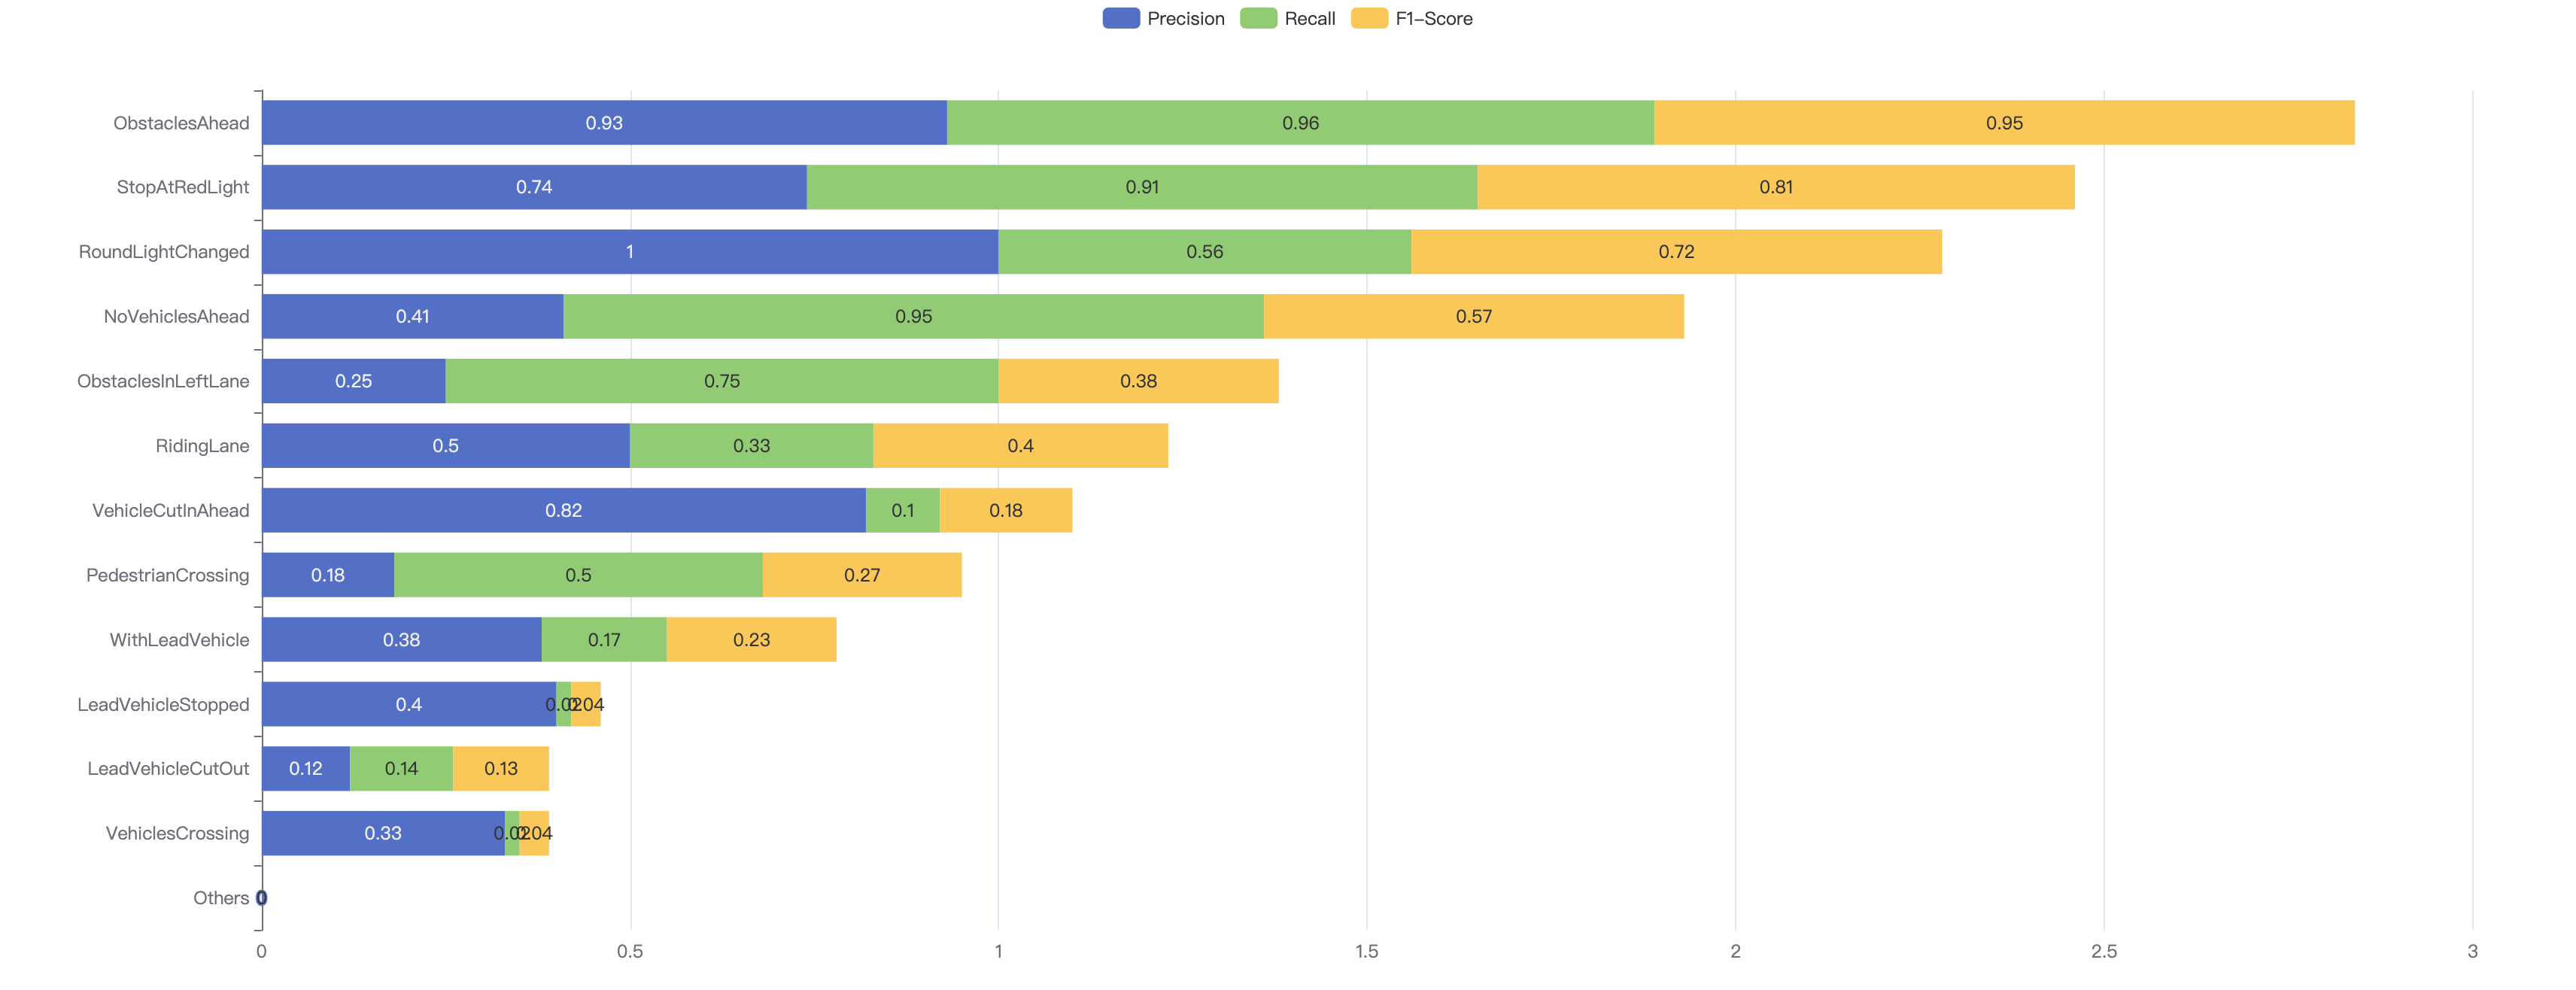
\includegraphics[width=1\linewidth]{images/result2.png}
    \caption{第二种问答生成三级标签的结果}
\end{figure}

\scriptsize
Others:LeadVehicleStopped, StopAtGreenLight, StopAtYellowLight, RidingLane, ArrowLightChanged, StopAtFlashGreenLight, VehiclesCrossing, LeadVehicleStppoed, LeadVehicleWrongDriveway
\normalsize

\end{frame}


\begin{frame}{第二种问答:错误分析}

\begin{minipage}[t]{0.4\textwidth}
  \centering
  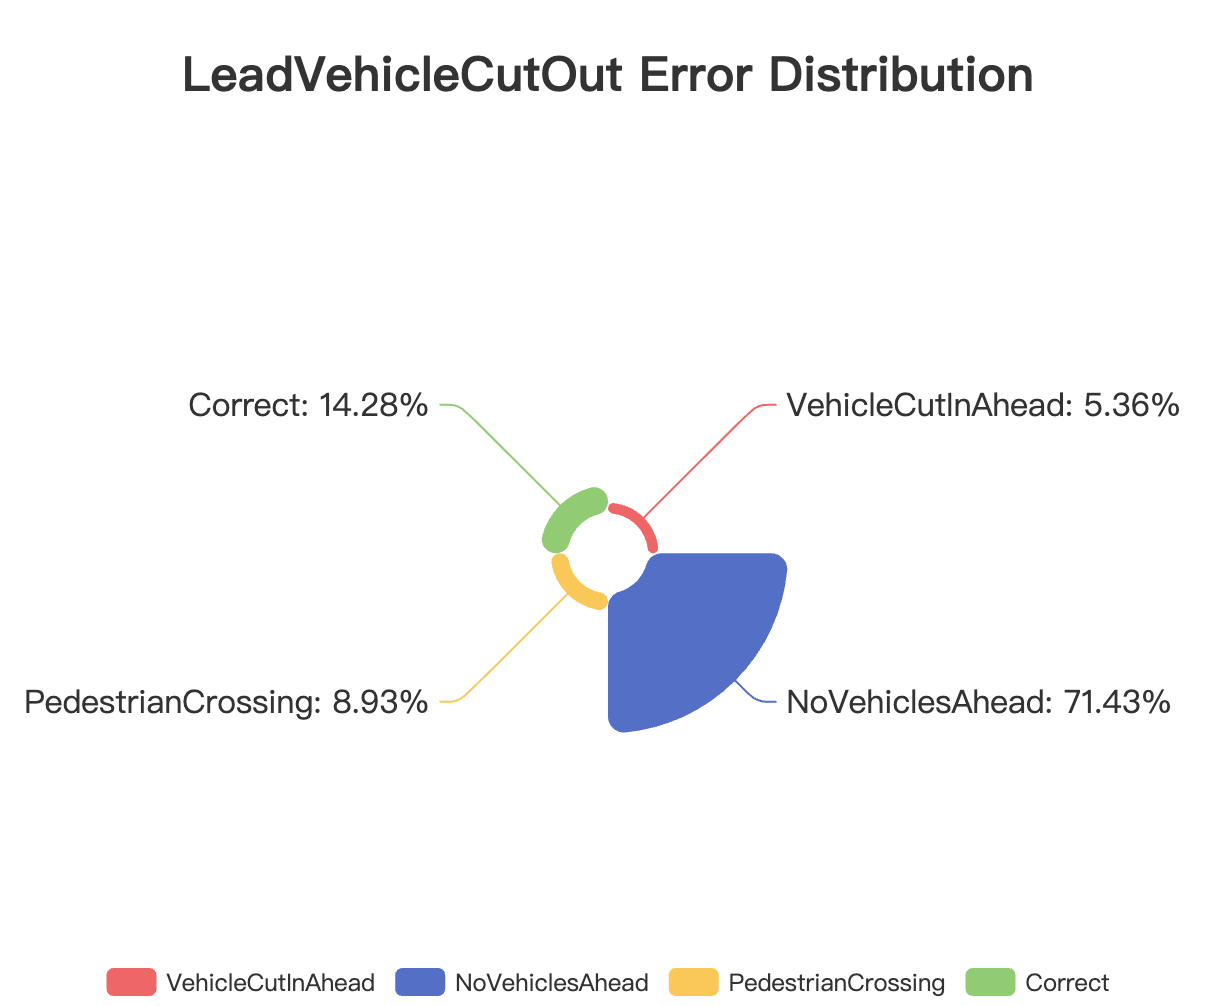
\includegraphics[width=\linewidth]{images/Q2 LeadVehicleCutOut Error Distribution.png}
\end{minipage}
\hfill
\begin{minipage}[t]{0.4\textwidth}
  \centering
  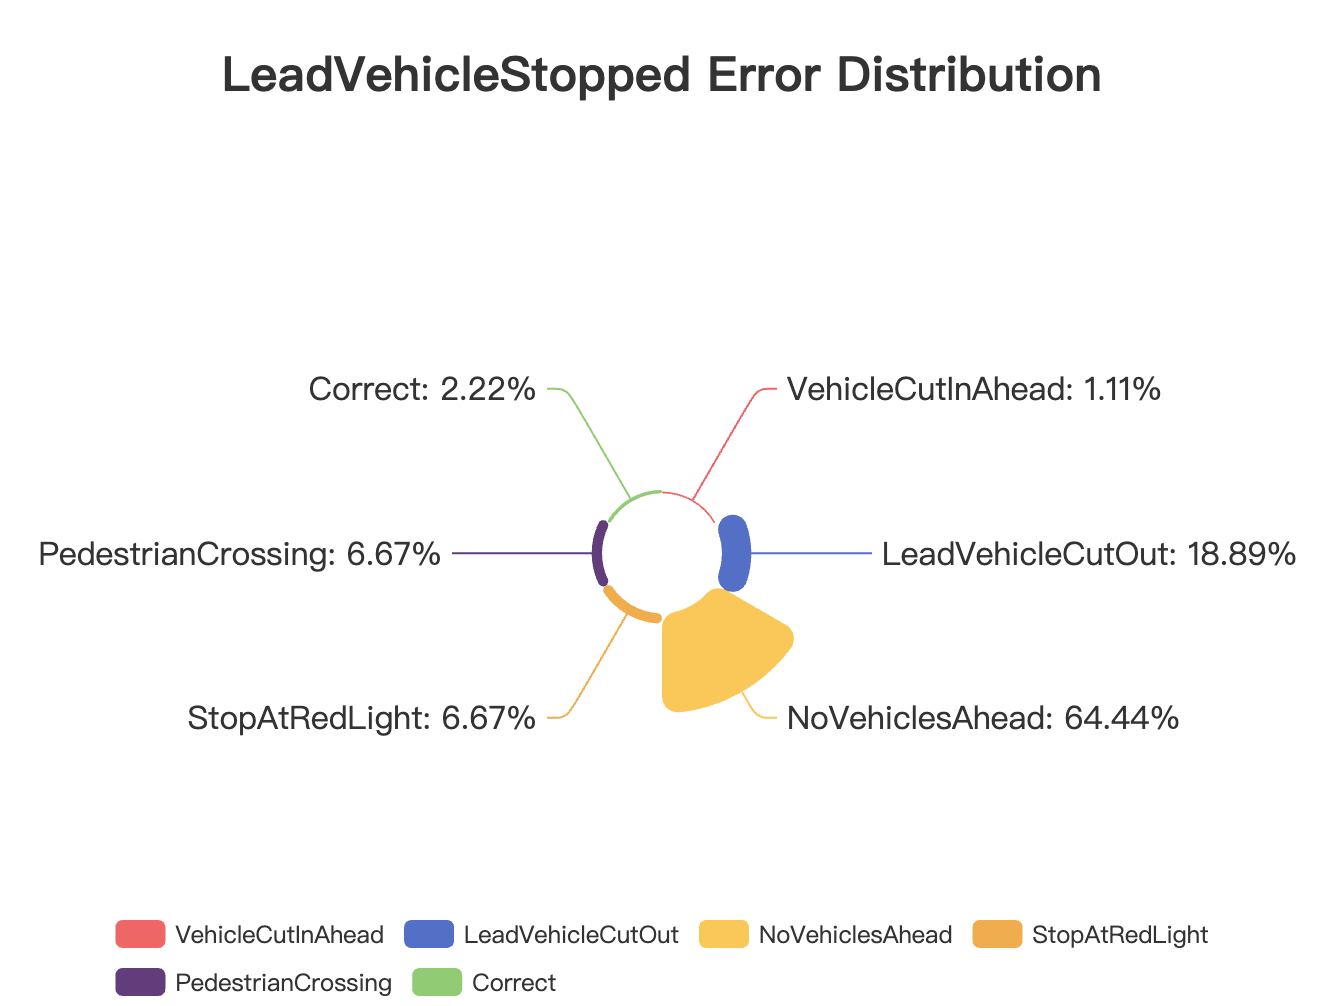
\includegraphics[width=\linewidth]{images/Q2 LeadVehicleStopped Error Distribution.png}
\end{minipage}


\begin{minipage}[t]{0.4\textwidth}
  \centering
  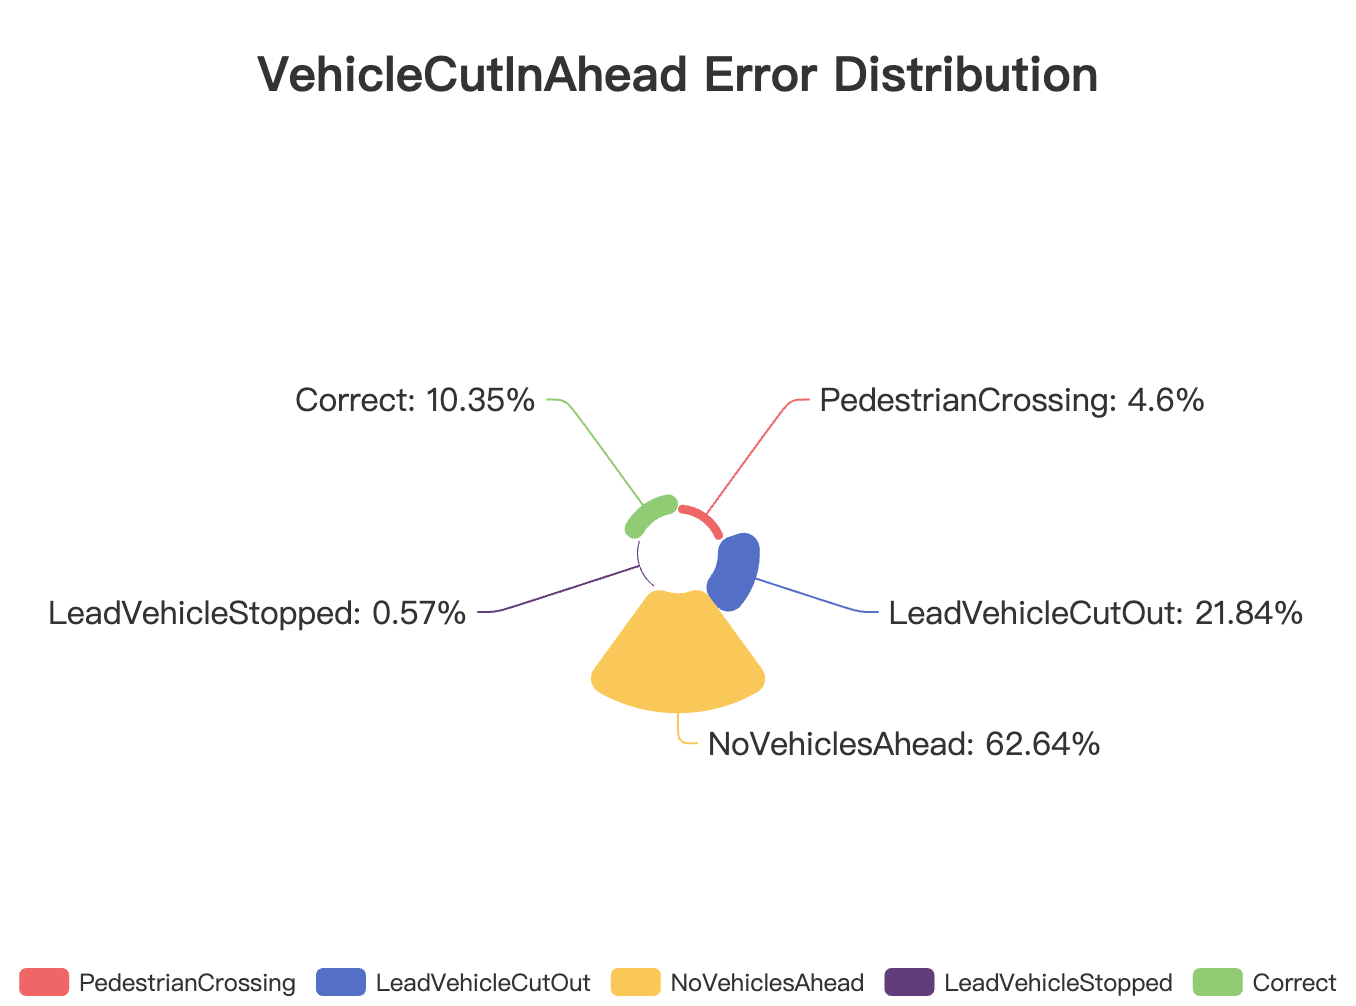
\includegraphics[width=\linewidth]{images/Q2 VehicleCutInAhead Error Distribution.png}
\end{minipage}
\hfill
\begin{minipage}[t]{0.4\textwidth}
  \centering
  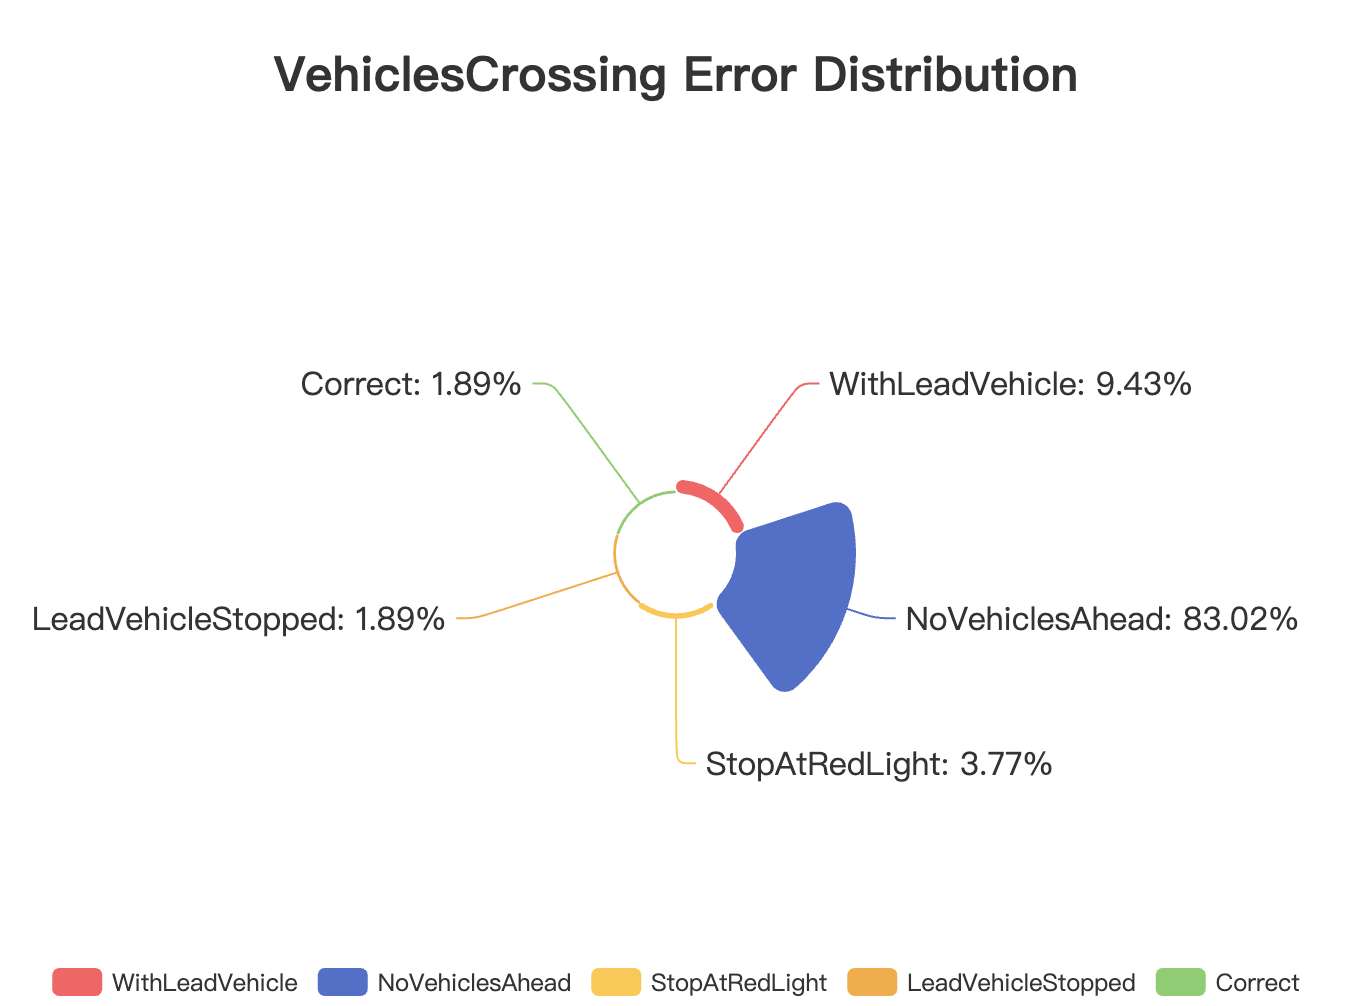
\includegraphics[width=\linewidth]{images/Q2 VehiclesCrossing Error Distribution.png}
\end{minipage}


\end{frame}

\begin{frame}{第三种问答设置(上)}
\scriptsize
\textbf{提问设计特点(1):}
\begin{itemize}
  \item 针对不同\textbf{二级标签}设计\textbf{个性化问题集合}
  \item 通过\textbf{分支式多轮问答}精准捕捉场景特征
  \item 充分利用二级标签语义,辅助更准确三级标签判定
\end{itemize}

\vspace{0.3em}
\textbf{二级标签与对应问题示例(1):}

\begin{itemize}
  \item \textbf{InLane}:
  \begin{itemize}
    \item Is there any \textcolor{red}{vehicle} in front of the ego vehicle?
    \item If there are \textcolor{red}{pedestrians crossing} in front of the ego vehicle, answer "pedestrian crossing". Otherwise skip.
    \item What does the \textcolor{red}{vehicle in front} do? \textcolor{red}{Change lanes}, \textcolor{red}{stop}, or \textcolor{red}{drive} in the opposite direction?
    \item If the vehicle in front \textcolor{red}{changes lanes}, does it \textcolor{red}{enter} the current lane (\textcolor{red}{cutting in}) or \textcolor{red}{leave} it (\textcolor{red}{cutting out})?
    \item Does the vehicle in front \textcolor{red}{stop}?
    \item Does the vehicle in front \textcolor{red}{drive} in the \textcolor{red}{opposite direction}?
  \end{itemize}
  
  \item \textbf{ChangingLaneLeft}:
  \begin{itemize}
    \item Are there \textcolor{red}{obstacles} ahead? Obstacles exclude vehicles and pedestrians (e.g., bicycles).
    \item If yes, are the obstacles in the \textcolor{red}{left lane} or \textcolor{red}{directly ahead}?
    \item If no obstacles, is the ego vehicle \textcolor{red}{riding the lane}?
  \end{itemize}

  \item \textbf{ChangingLaneRight}:
  \begin{itemize}
    \item Are there \textcolor{red}{obstacles} ahead? Exclude vehicles and pedestrians.
    \item If yes, are obstacles in the \textcolor{red}{right lane} or \textcolor{red}{directly ahead}?
    \item If no obstacles, is the ego vehicle \textcolor{red}{riding the lane}?
  \end{itemize}
\end{itemize}
\normalsize
\end{frame}


\begin{frame}{第三种问答设置(下)}
\scriptsize
\textbf{提问设计特点(2):}
\begin{itemize}
  \item 问题聚焦\textbf{驾驶行为、交通信号、行人与障碍物}等关键因素
\end{itemize}

\vspace{0.6em}
\textbf{二级标签与对应问题示例(2):}

\begin{itemize}
  \item \textbf{StopAndWait}:
  \begin{itemize}
    \item Is there a \textcolor{red}{traffic light} ahead?
    \item What is the \textcolor{red}{color} of the traffic light? \textcolor{red}{Red}, \textcolor{red}{Yellow} or \textcolor{red}{Green}?
    \item If no red light, are there \textcolor{red}{pedestrians crossing}?
    \item If no pedestrians, are there \textcolor{red}{vehicles crossing} ahead?
  \end{itemize}

  \item \textbf{Starting}:
  \begin{itemize}
    \item What color is the \textcolor{red}{traffic light}?
    \item Is the traffic light \textcolor{red}{changing}? If not, skip.
    \item What is the \textcolor{red}{shape} of the traffic light? \textcolor{red}{Round} or \textcolor{red}{Arrow}?
  \end{itemize}

  \item \textbf{EnterWaitingArea}:
  \begin{itemize}
    \item What is the \textcolor{red}{shape} of the traffic light? \textcolor{red}{Round} or \textcolor{red}{Arrow}?
  \end{itemize}

  \item \textbf{GoStraight / TurnLeft / TurnRight / UTurn}:
  \begin{itemize}
    \item Are there \textcolor{red}{vehicles} ahead or not during the maneuver?
    \item If yes, are the vehicles \textcolor{red}{leading} the ego vehicle or \textcolor{red}{crossing} in different directions?
  \end{itemize}
\end{itemize}
\normalsize
\end{frame}

\begin{frame}{第三种问答结果}

\begin{figure}
    \centering
    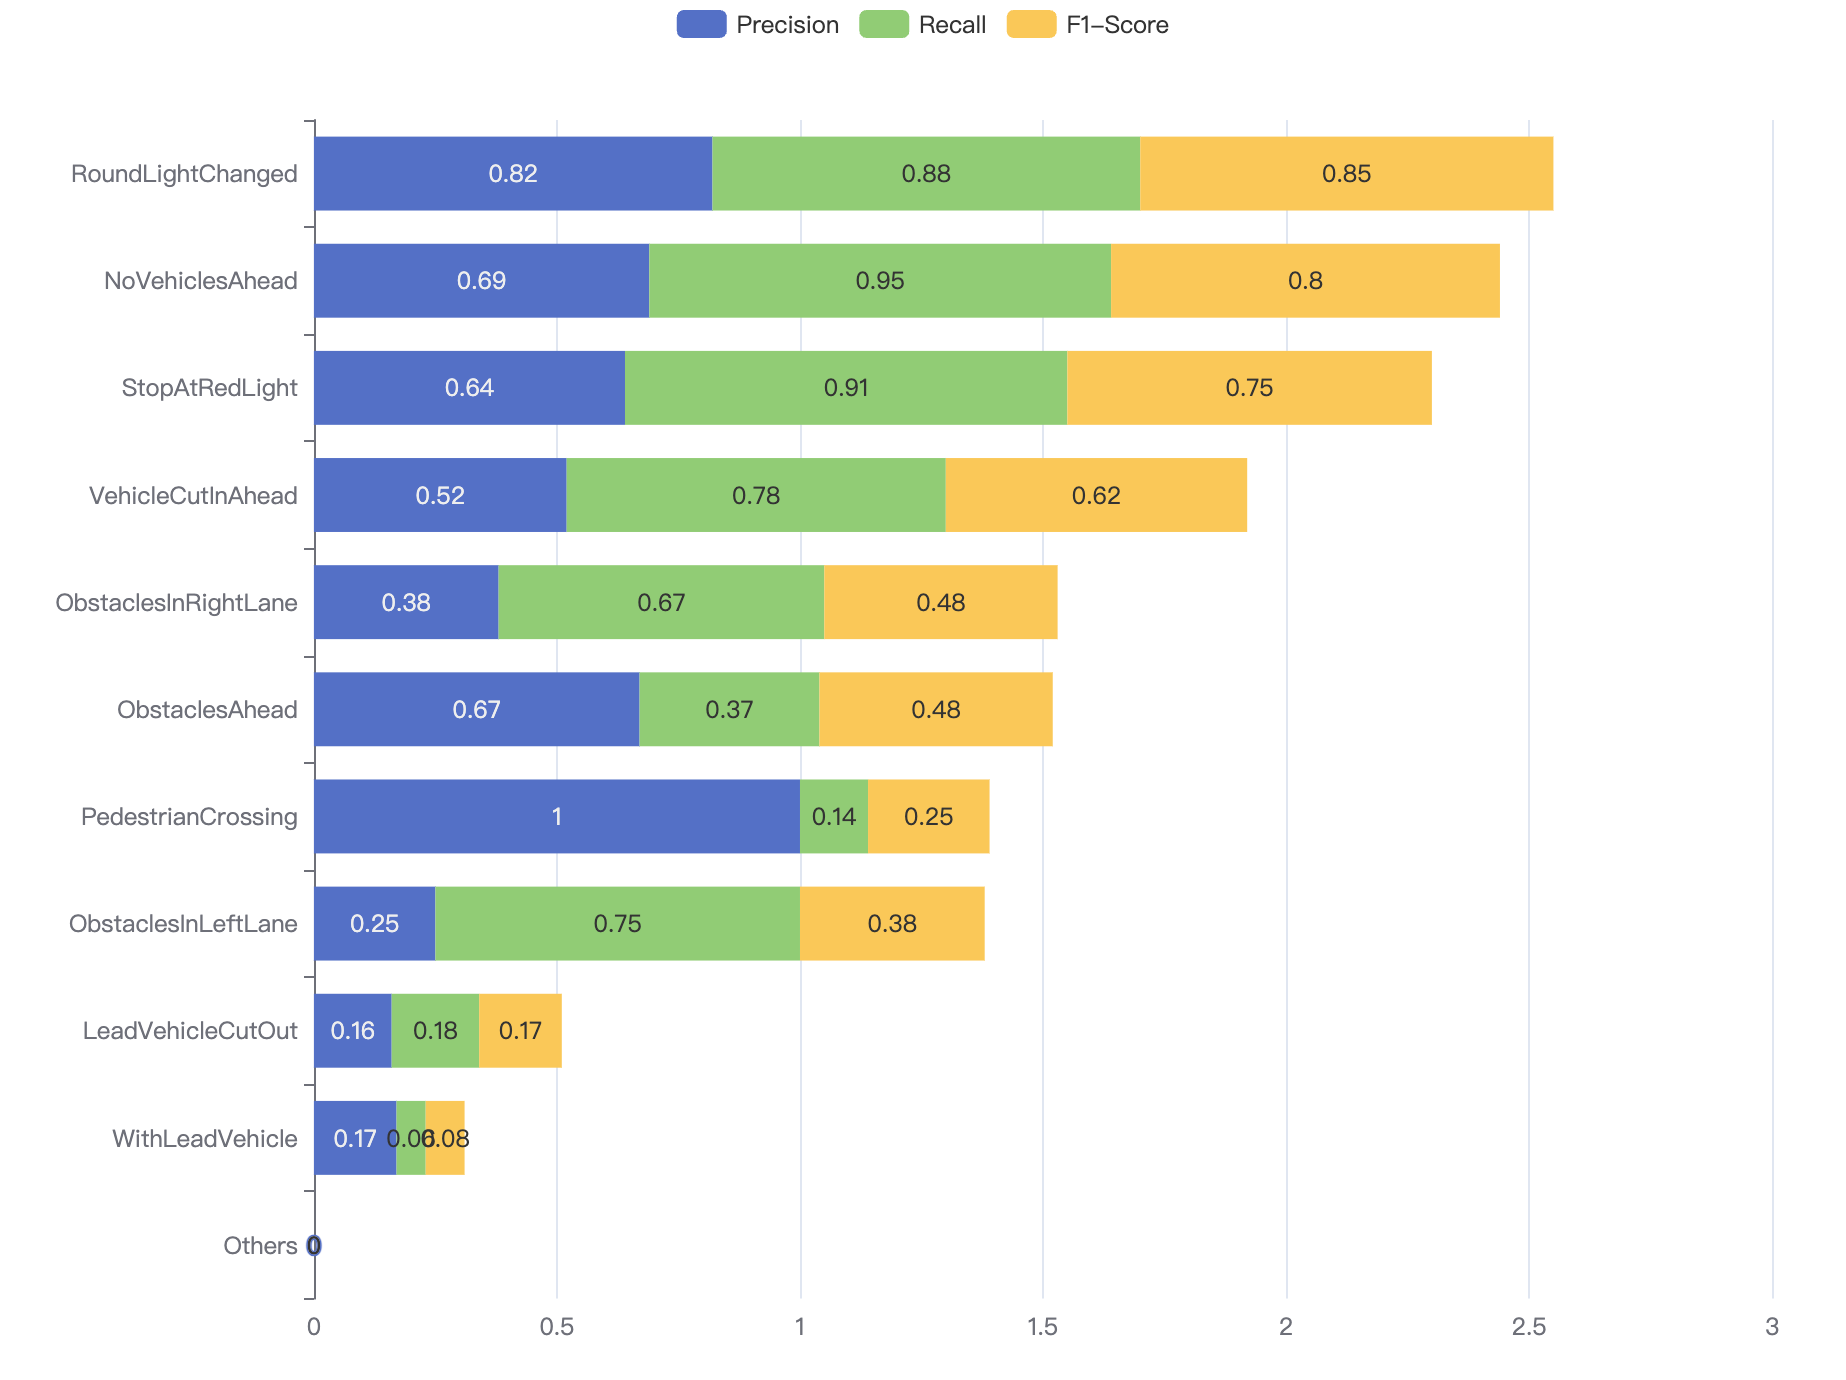
\includegraphics[width=1\linewidth]{images/result3.png}
    \caption{第二种问答生成三级标签的结果}
\end{figure}


\scriptsize
Others:LeadVehicleStopped, LeadVehicleStppoed, LeadVehicleWrongDriveway, RidingLane, StopAtFlashGreenLight, StopAtGreenLight, StopAtYellowLight, VehiclesCrossing, ArrowLightChanged
\normalsize
\end{frame}


\begin{frame}{第三种问答:错误分析}

\begin{minipage}[t]{0.4\textwidth}
  \centering
  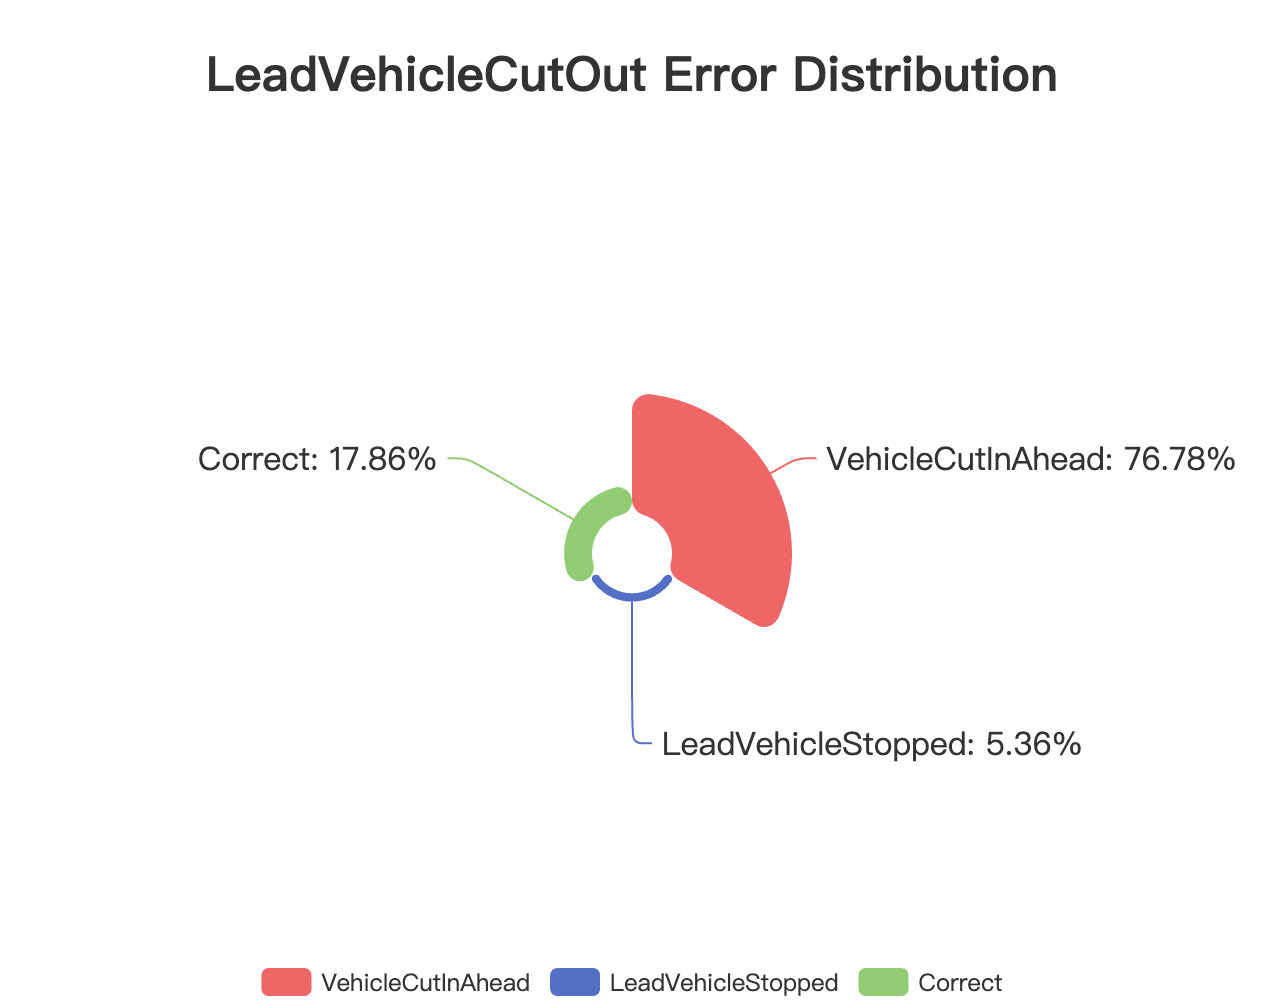
\includegraphics[width=\linewidth]{images/Q3 LeadVehicleCutOut Error Distribution.png}
\end{minipage}
\hfill
\begin{minipage}[t]{0.4\textwidth}
  \centering
  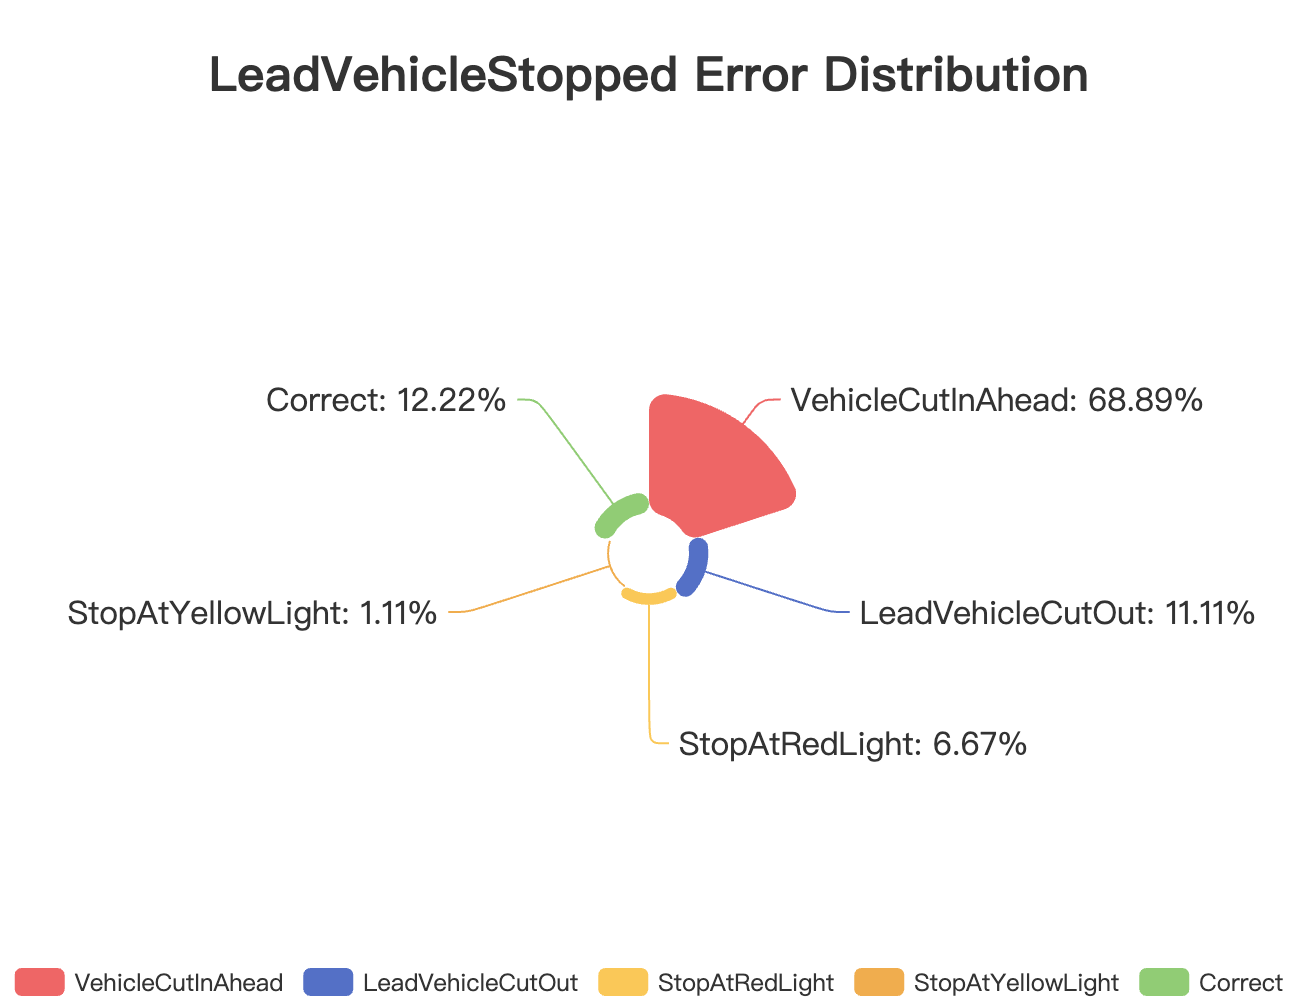
\includegraphics[width=\linewidth]{images/Q3 LeadVehicleStopped Error Distribution.png}
\end{minipage}


\begin{minipage}[t]{0.4\textwidth}
  \centering
  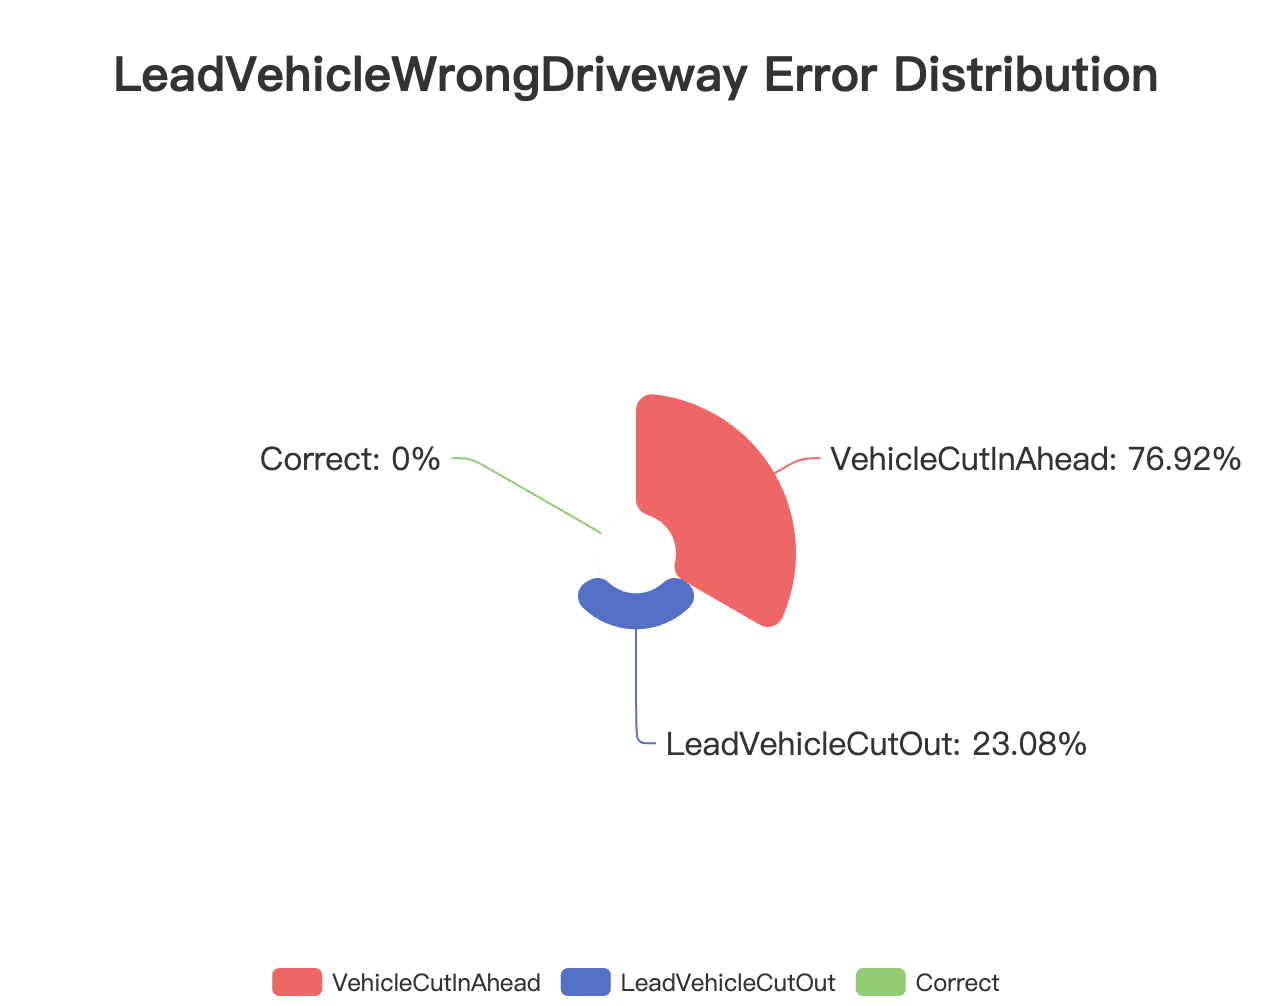
\includegraphics[width=\linewidth]{images/Q3 LeadVehicleWrongDriveway Error Distribution.png}
\end{minipage}
\hfill
\begin{minipage}[t]{0.4\textwidth}
  \centering
  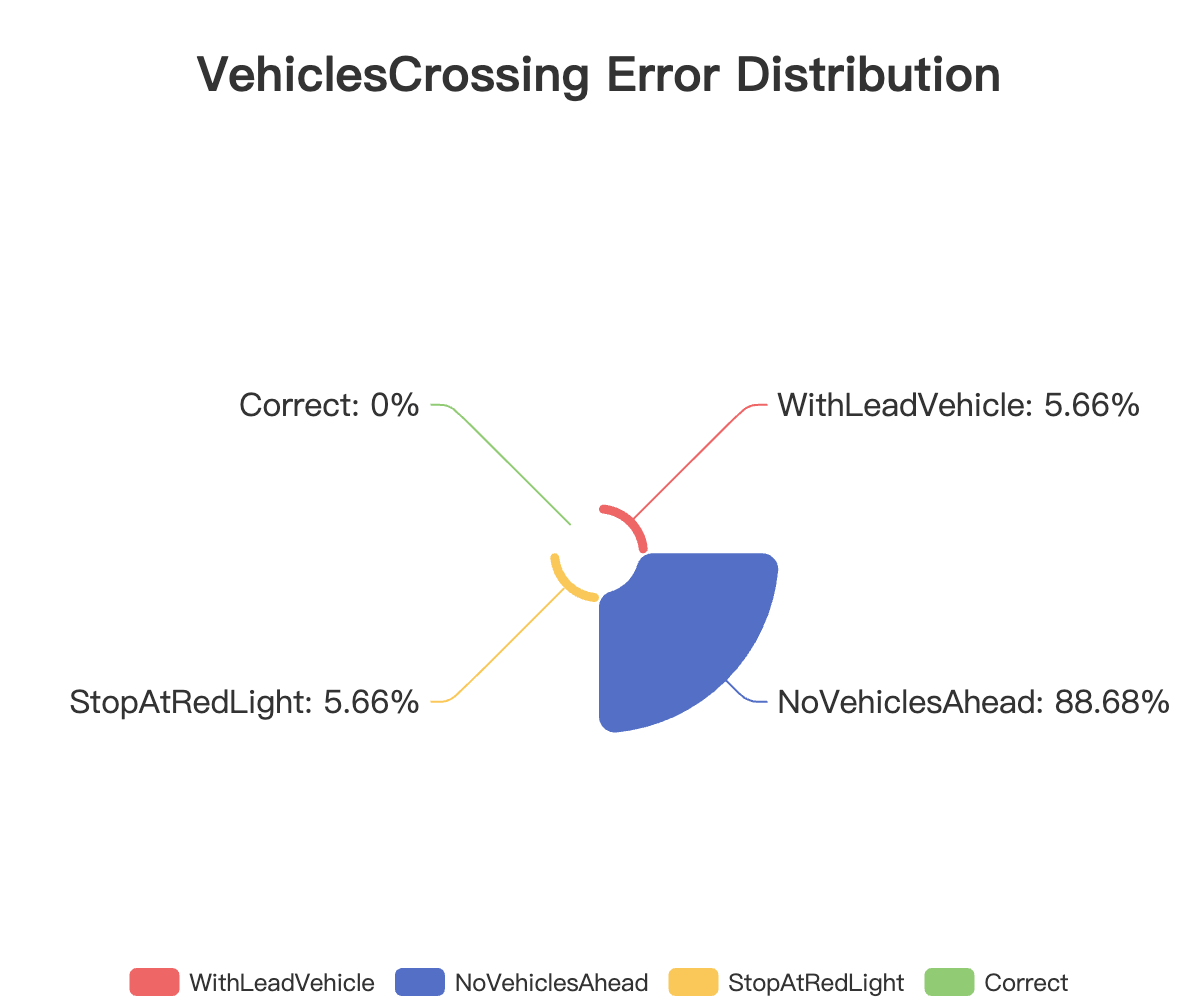
\includegraphics[width=\linewidth]{images/Q3 VehiclesCrossing Error Distribution.png}
\end{minipage}


\end{frame}
%--------------------------------------------

\section{多模态大语言模型(MLLM)模型微调}
\begin{frame}{微调目的与挑战}
\begin{itemize}
  \item \textbf{当前模型表现不足}:
    \begin{itemize}
      \item 对于 \textbf{LeadVehicleCutOut} 识别较差,易混淆为 \textbf{VehicleCutInAhead};
      \item \textbf{VehiclesCrossing}、\textbf{LeadVehicleStopped} 等标签表现不佳,反映模型\textbf{对方向及相对运动关系理解不足};
      \item 信号灯等\textbf{细节识别能力有限},影响准确语义理解。
    \end{itemize}

  \item \textbf{引入思维链推理的意义}:
    \begin{itemize}
      \item 强化模型对 \textbf{位置关系}和 \textbf{运动状态}的推理能力;
      \item 利用多轮交互式问答方式引导模型逐步细化理解;
      \item 思维链方法已被验证能显著提升复杂任务的语言模型表现。
    \end{itemize}

  \item \textbf{微调的优势}:
    \begin{itemize}
      \item 在\textbf{自动驾驶场景特定数据}上增强语义理解的准确性和鲁棒性;
      \item 促进模型更精准捕捉动态交互及细节信息;
      \item 提升视频-文本检索等下游任务的整体效果。
    \end{itemize}
\end{itemize}
\end{frame}


\begin{frame}[fragile]{微调数据组织:基于思维链结构}
模仿\textbf{DriveLM思维链}结构,将微调数据组织为\textbf{层次化、多轮交互问答}形式,便于模型逐步推理视频中的关键语义信息:

\begin{itemize}
  \item 每条对话包含\textbf{多轮问答},逐层捕捉感知(Perception)、预测(Prediction)、规划(Planning)、行为(Behavior)、运动(Motion)等阶段信息
  \item \textbf{区分问题类型},辅助模型理解时序与逻辑依赖
  \item 增强模型对细节和复杂场景的理解与推理能力
\end{itemize}

\vspace{-0.5em}
\begin{figure}
    \centering
    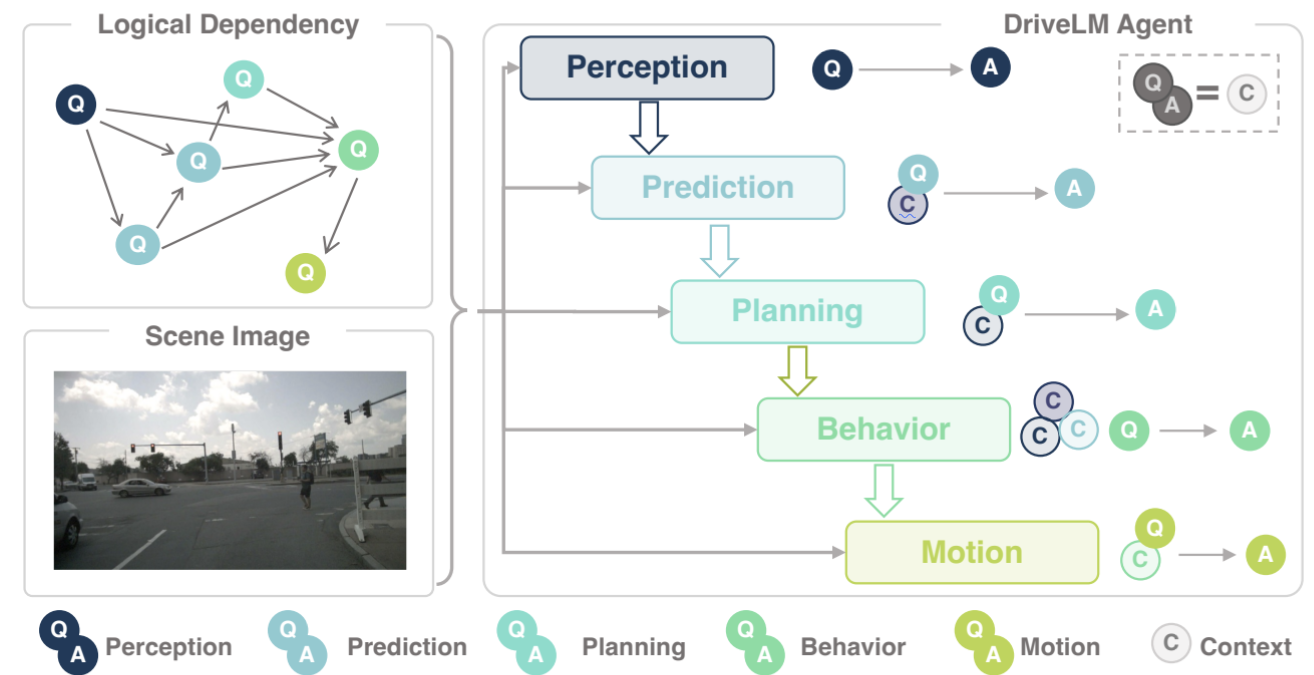
\includegraphics[width=0.6\linewidth]{images/CoT.png}
    \caption{Chain of Thought in DriveLM}
    \label{fig:Chain of Thought in DriveLM}
\end{figure}

\end{frame}


\begin{frame}{微调数据组织示例}

示例对话(括号内为思维链阶段注释):

\scriptsize
\begin{tcolorbox}[listing only, listing options={
    language=,
    basicstyle=\ttfamily\tiny,
    escapeinside={(*@}{@*)}
}]
human: <image> What objects are detected in front of the ego vehicle? (\textcolor{blue}{Perception})

gpt: There is a stopped vehicle and a pedestrian crossing ahead.

\vspace{6pt}
human: <image> Based on current speed and positions, will the pedestrian cross the road in front of the ego vehicle? (\textcolor{blue}{Prediction})

gpt: Yes, the pedestrian is moving towards the crosswalk and will cross soon.

\vspace{6pt}
human: <image> Is the ego vehicle planning to stop or slow down for the pedestrian? (\textcolor{blue}{Planning})

gpt: The ego vehicle is planning to slow down to yield to the pedestrian.

\vspace{6pt}
human: <image> Is the ego vehicle currently slowing down? (\textcolor{blue}{Behavior})

gpt: Yes, the ego vehicle is reducing speed gradually.

\vspace{6pt}
human: <image> Is the ego vehicle maintaining lane position during this maneuver? (\textcolor{blue}{Motion})

gpt: Yes, the vehicle remains centered in its lane while slowing down.
\end{tcolorbox}


\normalsize
\vspace{0.5em}
通过\textbf{分阶段、分步骤问答}组织微调数据,帮助模型逐步推理环境信息
\end{frame}


\begin{frame}{微调后模型效果}

\noindent
\begin{minipage}[t]{0.48\textwidth}
  \centering
  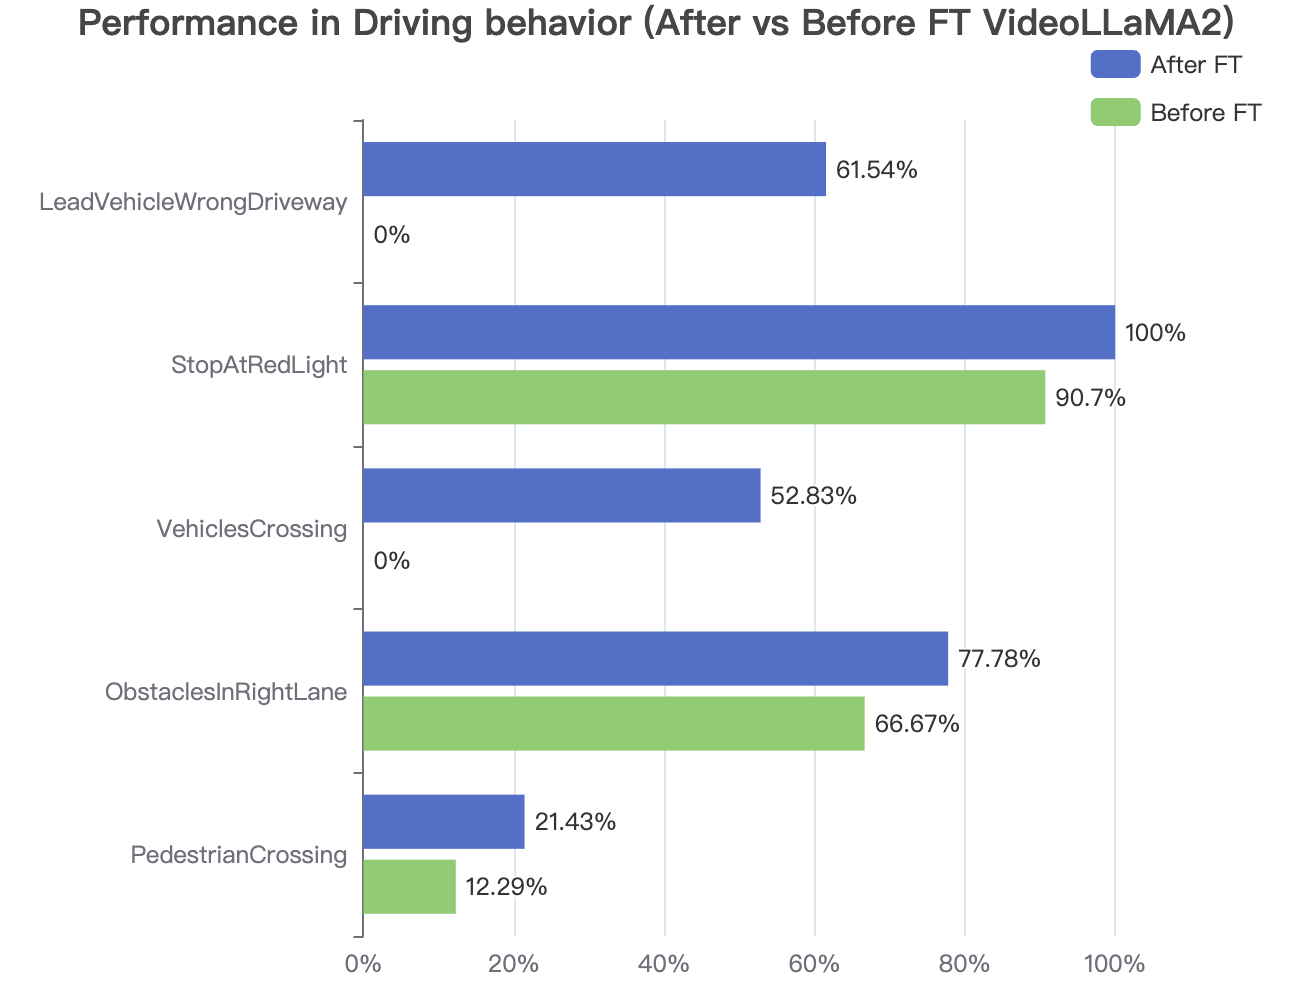
\includegraphics[width=\linewidth]{images/Performance in Driving behavior(VideoLLaMA2).png}
  \caption{VideoLLaMA2微调效果}
\end{minipage}
\hfill
\begin{minipage}[t]{0.48\textwidth}
  \centering
  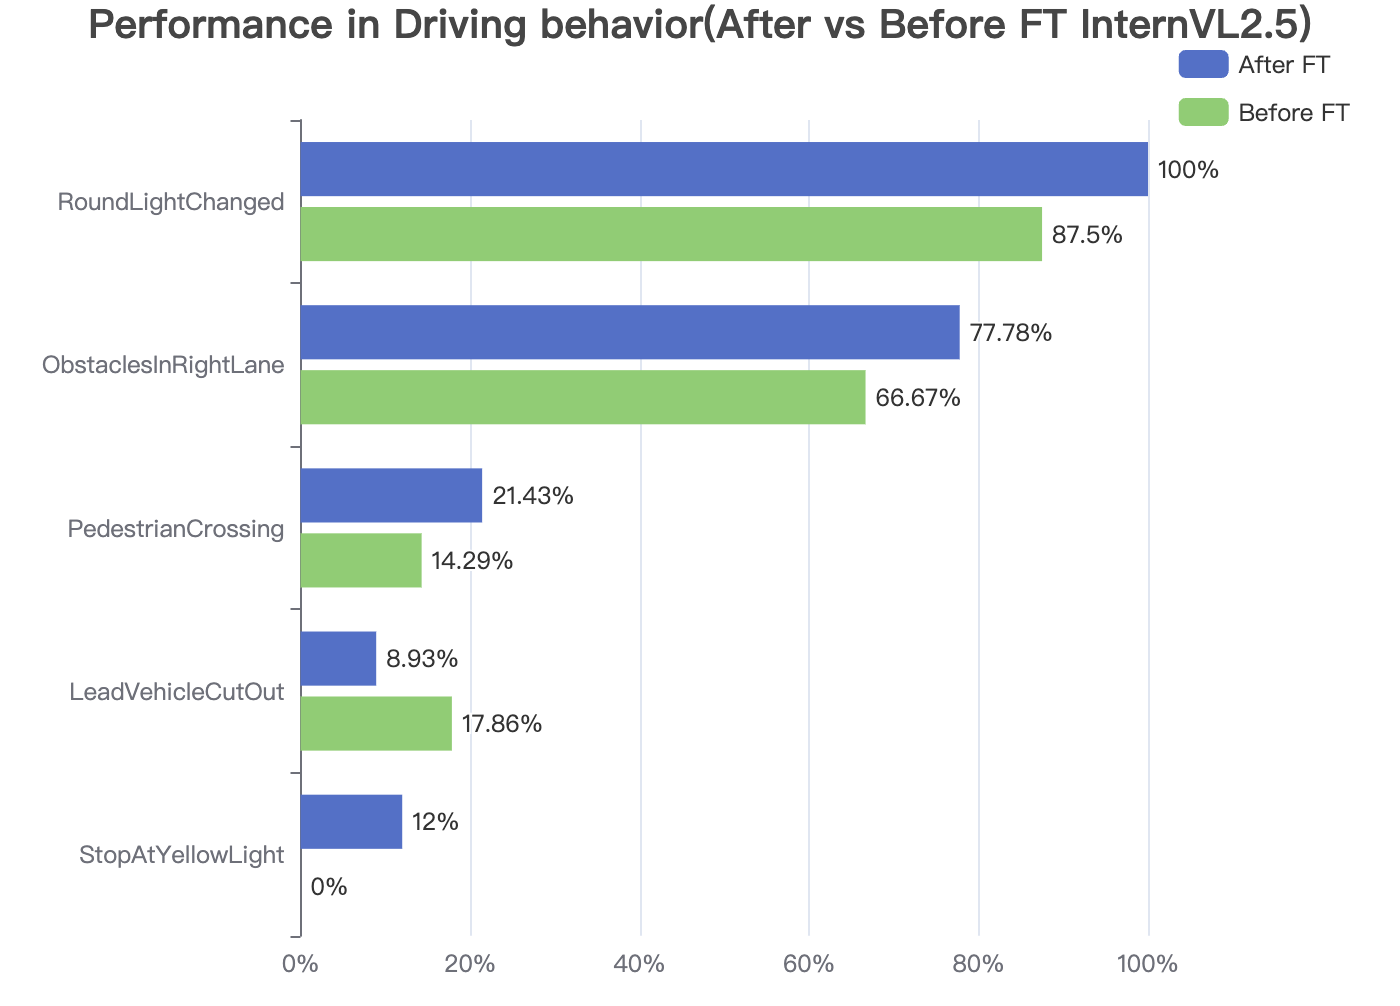
\includegraphics[width=\linewidth]{images/Performance in Driving behavior(InternVL2.5).png}
  \caption{InternVL2.5微调效果}
\end{minipage}

\vspace{1em}

\begin{itemize}
    \item 微调后\textbf{部分行为正确率提升}
    \item 尤其在\textbf{信号灯等细节判断、部分交互场景}的理解能力上均有明显改进。
\end{itemize}

\end{frame}

\section{后续计划}

\begin{frame}{动态知识蒸馏框架(DLDKD)简介}

\scriptsize
\begin{itemize}
  \item DLDKD:基于\textbf{动态知识蒸馏}的\textbf{多模态模型训练框架},旨在提升学生模型\textbf{对视频-文本相似度的理解能力}
  \item 其核心思想是\textbf{结合Teacher和Student模型},动态调整的知识蒸馏权重,引导学生学习教师模型的特征分布
  \item 教师模型:采用CLIP图像编码器和文本编码器
  \item 学生模型:双分支结构,分别继承和探索教师模型的知识;Transformer和注意力机制实现视频和文本的多模态融合。
  \item 动态权重的设计使模型在训练过程中,更好地捕捉\textbf{不同时间步的知识分布},提高蒸馏效果和泛化能力。
\end{itemize}

\normalsize
\centering
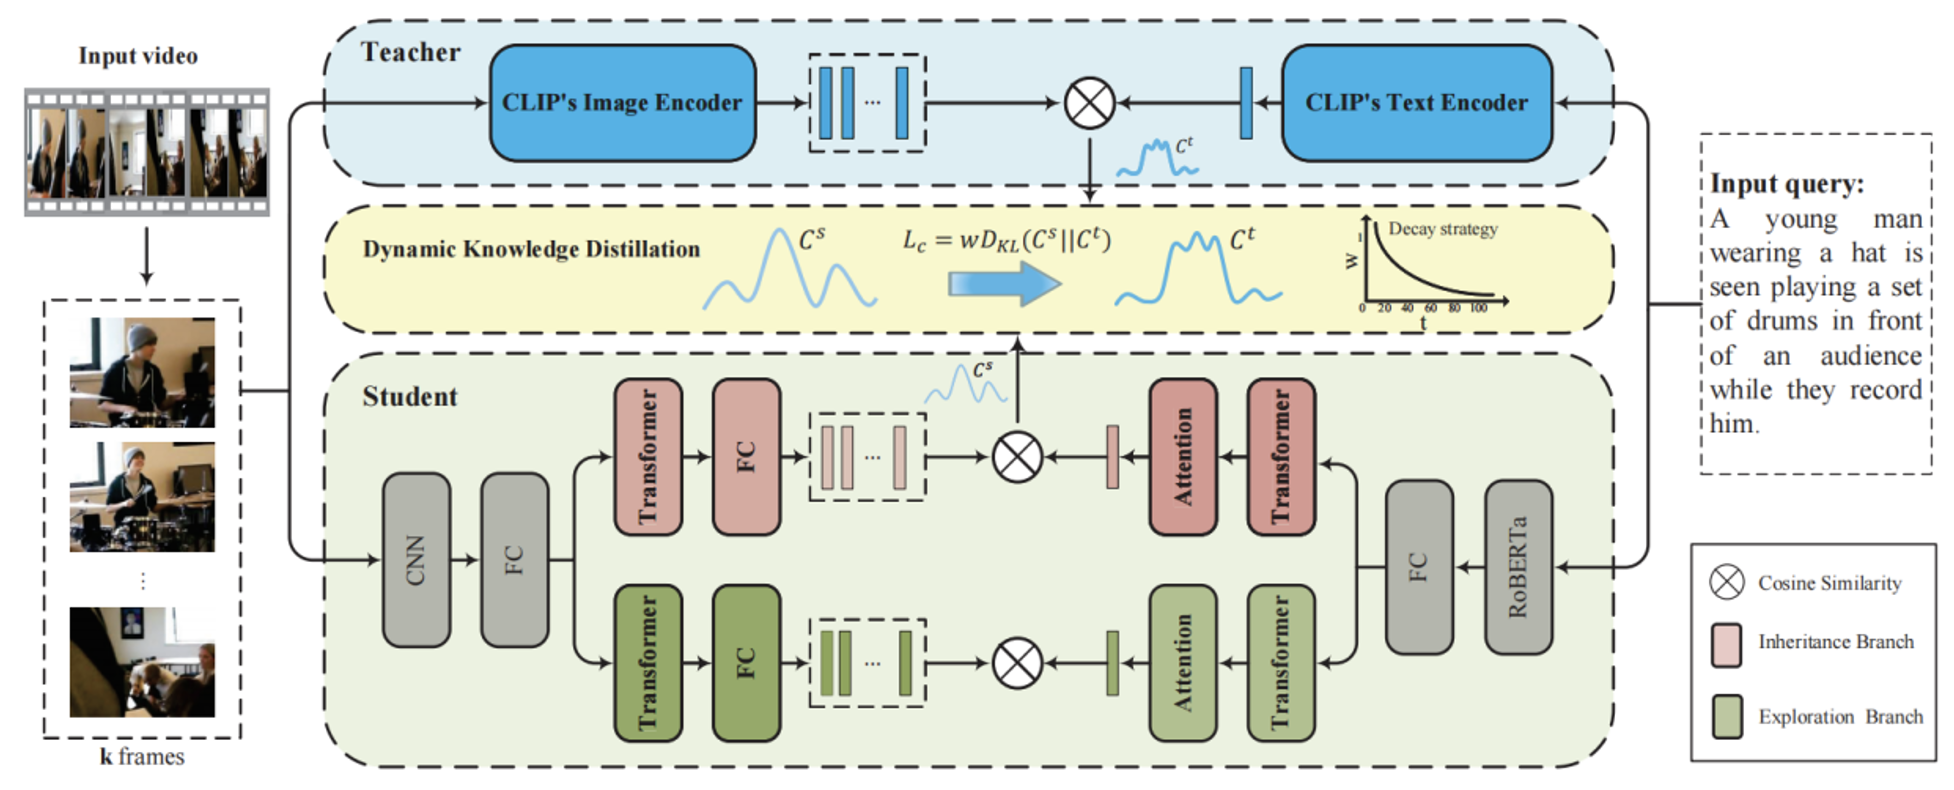
\includegraphics[width=0.8\linewidth]{images/DLDKD structure.png}
\end{frame}


\begin{frame}{后续计划:蒸馏VideoLLaMA2与InternVL模型}

\begin{itemize}
  \item \textbf{目标}:
  
  利用DLDKD框架,将大型预训练模型VideoLLaMA2和InternVL的知识蒸馏到\textbf{轻量级}学生模型中,提高自动驾驶场景下的视频-文本理解和检索性能
  \item \textbf{具体做法}:
    \begin{itemize}
      \item 以VideoLLaMA2和InternVL作为\textbf{教师模型},分别提供视觉和文本的特征表示
      \item 构建\textbf{双分支学生模型},融合视觉与文本信息,并采用Transformer和注意力机制增强多模态交互
      \item 设计动态知识蒸馏权重,结合教师模型的时间动态特征,指导学生模型逐步学习
      \item 结合自动驾驶数据集,针对\textbf{特定场景}进行微调和评估,提升模型在复杂环境下的推理和理解能力
    \end{itemize}
  \item \textbf{预期效果}:提升学生模型对\textbf{细节、时序和语义关系}的理解能力,实现\textbf{更准确的视频-文本匹配与语义检索}
\end{itemize}

\end{frame}

\end{document}